% libroResMat2
% Copyright (C) 2020  J.M. Perez Zerpa, et. al.
%
% This program is free software: you can redistribute it and/or modify
% it under the terms of the GNU General Public License as published by
% the Free Software Foundation version 3 of the License.
%
% This program is distributed in the hope that it will be useful,
% but WITHOUT ANY WARRANTY; without even the implied warranty of
% MERCHANTABILITY or FITNESS FOR A PARTICULAR PURPOSE. See the
% GNU General Public License for more details.
%
% You should have received a copy of the GNU General Public License
% along with this program.  If not, see <http://www.gnu.org/licenses/>.

\chapter{Soluciones de los ejercicios}

\section{Ejercicios de la UT1}

\begin{description}
\item [1.1] 
\begin{enumerate}[label=\alph*)]
\item Diagrama de cortantes en kN

\begin{center}
	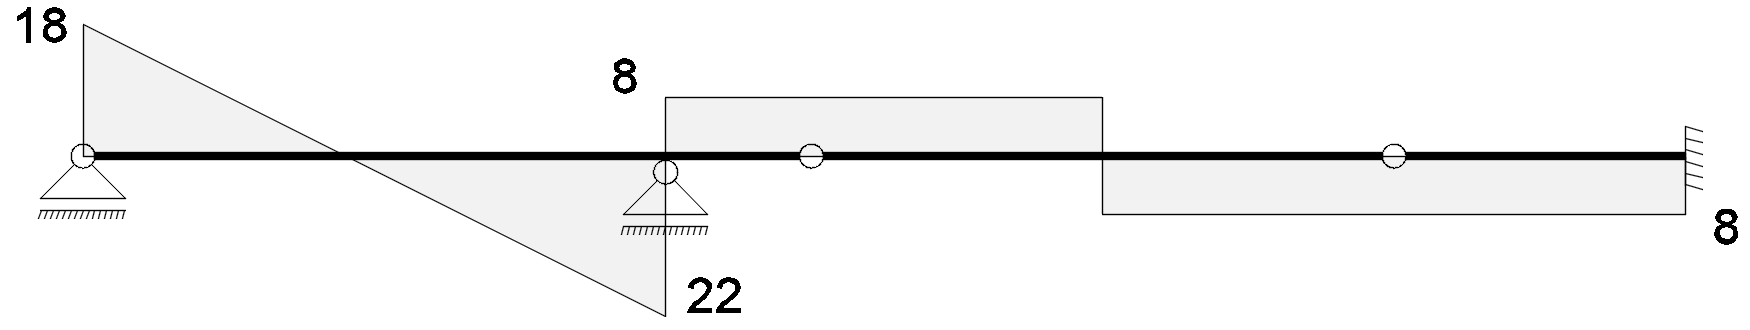
\includegraphics[width=.85\textwidth]{ej11a}
\end{center}

Diagrama de momentos en kNm

\begin{center}
	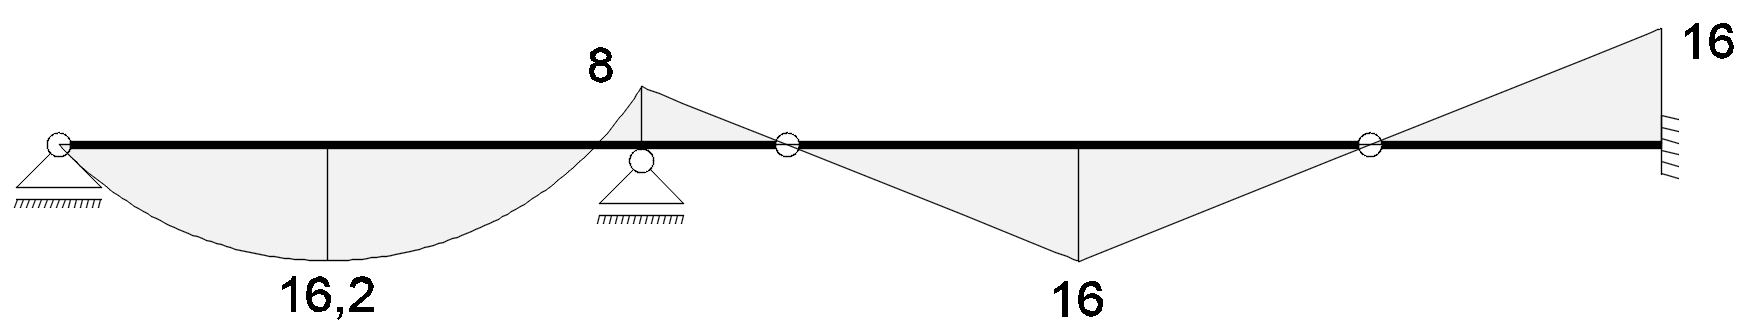
\includegraphics[width=.85\textwidth]{ej11b}
\end{center}

\item  $b = 15$ cm.
\item
\begin{itemize}
	\item $\theta_A = 6.32 \times 10^{-3}$ rad  horario,
	\item $\theta_B = 4.74 \times 10^{-3}$ rad antihorario,
	\item $\delta_C = 3.95 \times 10^{-3}$ m hacia arriba.
\end{itemize}

\end{enumerate}

\item[1.2] 

\begin{enumerate}[label=\alph*)]
	\item Directas en kN


\begin{center}
	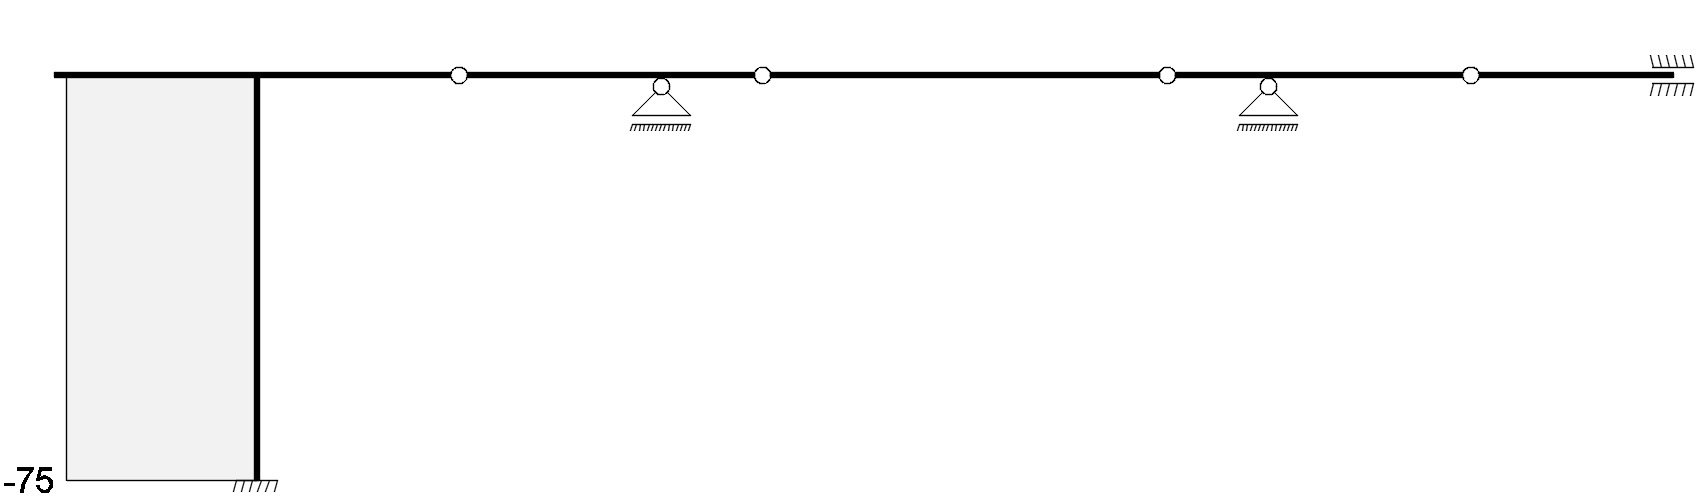
\includegraphics[width=.85\textwidth]{12a}
\end{center}

cortantes en kN

\begin{center}
	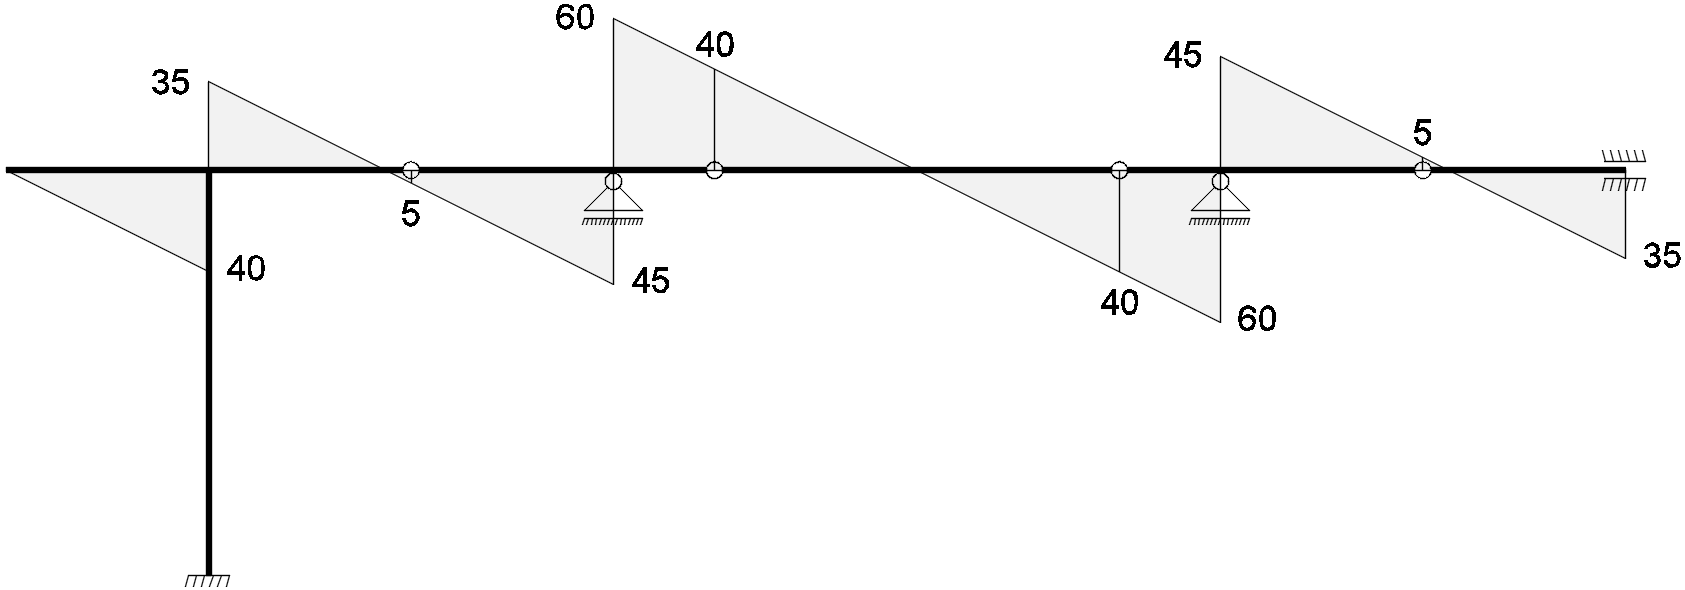
\includegraphics[width=.85\textwidth]{12b}
\end{center}

momentos en kN m

\begin{center}
	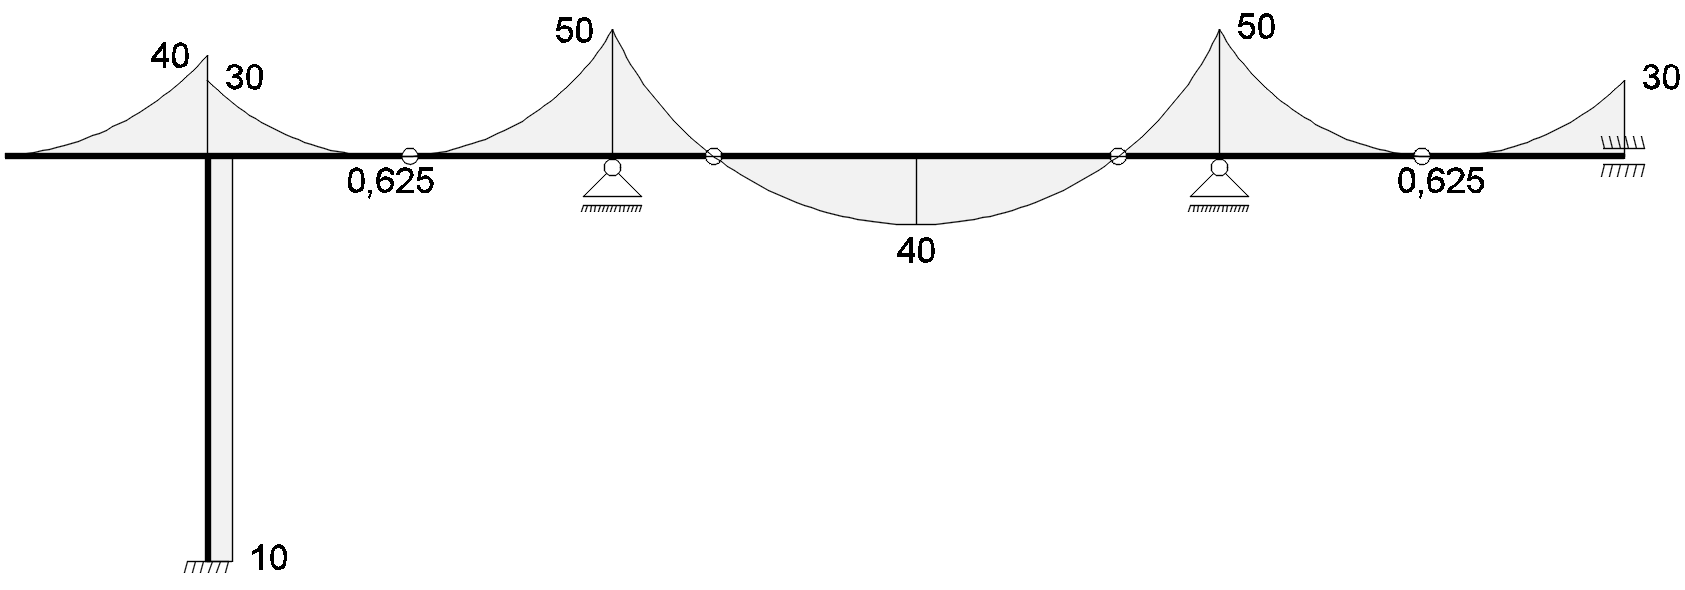
\includegraphics[width=.85\textwidth]{12c}
\end{center}
\addtocounter{enumi}{1}

\item 
\begin{itemize}
\item $\theta_D = (53.33$ kN m$^2)$/EI horario.
\item $ \theta_G = (13.33$ kN m$^2)$/EI antihorario.
\item $ \delta_C = (53.33 $ kN m$^3)$/EI hacia arriba y $(80$ kN m$^3)$/EI hacia la izquierda.
\item  $\delta_H = (26.67$ kN m$^3)$/EI hacia abajo y $(80$ kN m$^3)$/EI hacia la izquierda.
\end{itemize} 
\end{enumerate}

%
\item[1.3]

\begin{enumerate}[label=\alph*)]
	
\item $P = +210$ kN / $- 163.3$ kN.

\item $2$ PNC $6.5$.

\end{enumerate}
	%
\item [1.4]


a)

	\begin{center}
		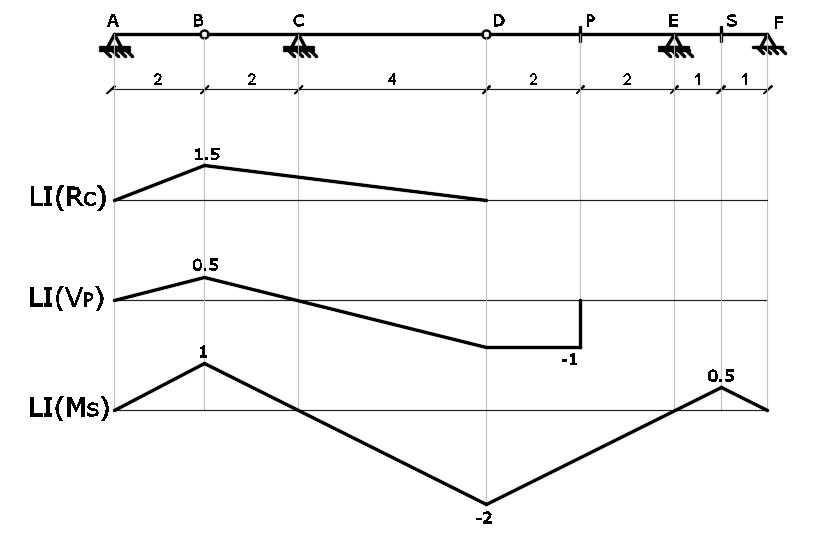
\includegraphics[width=.85\textwidth]{14a}
	\end{center}
b)
\begin{itemize}
\item RC
\begin{itemize}
	\item Máximo: De A a D $\rightarrow$ RC,MAX = 120 kN.
    \item Mínimo: Sin carga $\rightarrow$ RC,MIN = 0 kN.
    \end{itemize}
\item VP
\begin{itemize}
	\item Máximo: De A a C $\rightarrow$ VC,MAX= 20 kN.
    \item Mínimo: De C a P $\rightarrow$ VC,MIN = -80 kN.
    \end{itemize}
\item MS
\begin{itemize}
	\item Máximo: De A a C y de E a F $\rightarrow$ MC,MAX = 50 kN m.
   \item Mínimo: De C a E $\rightarrow$ MC,MIN = -160 kN m.
\end{itemize}
\end{itemize}

\item [1.5]
%
Reacciones,
\begin{itemize}
\item MA = $-5.2$ kN m.
\item  RA = $5.04$ kN.
\item RB $= 24.96$ kN + 40 kN  $= 64.96$ kN.
\end{itemize}
%


Cortante en kN

\begin{center}
	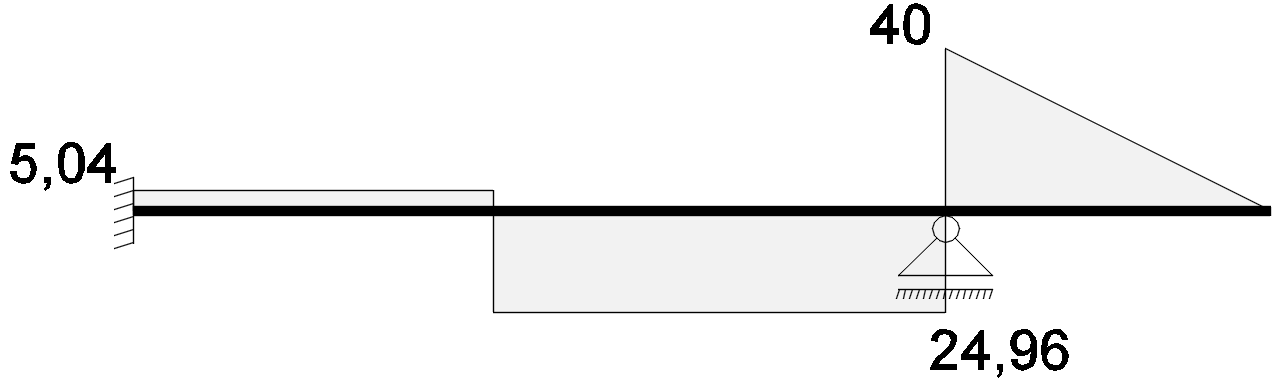
\includegraphics[width=.65\textwidth]{15a}
\end{center}

Momentos en kN m
 
 \begin{center}
 	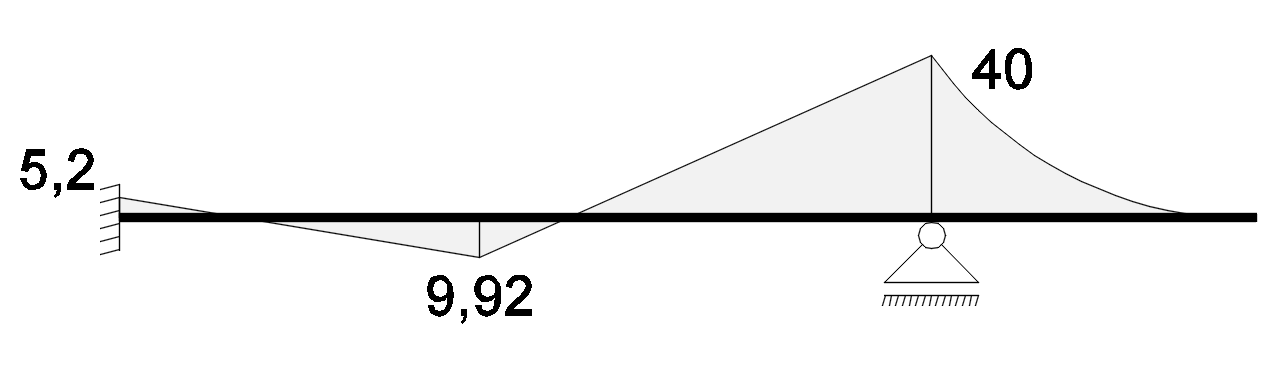
\includegraphics[width=.65\textwidth]{15b}
 \end{center}

\end{description}



\section{Ejercicios de la UT2}




\begin{description}
\item [2.1]
%
Reacciones
\begin{itemize}
\item RB = 50 kN hacia la izquierda y 50 kN hacia abajo.
\item RC = 50 kN hacia arriba.
\end{itemize}


Directas en barras
\begin{center}
\begin{tabular}{lr}
\hline
Barra & N [kN] \\
\hline
AB & 50 \\
BC & 0 \\
AC & $-70.7$\\
\hline
\end{tabular}
\end{center}

Desplazamiento de A: $2.44 \times  10^{-3}$ m hacia la derecha y $6.38 \times 10^{.4}$ m hacia arriba.

%
\item [2.2]

Reacciones
\begin{itemize}
\item RA = 13,48 kN hacia abajo (reacción horizontal en A nula).
\item RB = 33,04 kN hacia abajo.
\item  RC = 106,52 kN hacia arriba.
\end{itemize}

Directas en barras
\begin{center}
	\begin{tabular}{lr}
		\hline
Barra & N [kN] \\
\hline
AB & $-18.0$ \\
AE & $22.5$ \\
BE & $46.5$ \\
BC & $-22.5$ \\
EC & $-62.0$ \\
EF & $100.0$ \\
CF & $-60.0$ \\
CD & $-100.0$ \\
FD & $80.0$ \\
\hline
\end{tabular}
\end{center}

Desplazamiento de D: $ 2.15 \times 10^{-3}$ m hacia la derecha y $4.8 \times 10^{-3}$ m hacia abajo.

\item[2.3]

Reacciones
\begin{itemize}
\item RA = 20 kN hacia la izquierda.
\item RD = 20 kN hacia la derecha y 10 kN hacia arriba.
\end{itemize}

\begin{center}
	\begin{tabular}{lr}
		\hline
		Barra & N [kN] \\
		\hline
AB & $15.68$ \\
BC & $4.42$ \\
AD & $-4.42$ \\
BE & $0.00$ \\
CF & $4.42$ \\
AE & $6.25$ \\
DB & $-7.89$ \\
BF & $7.89$ \\
CE & $-6.25$ \\
DE & $-14.42$ \\
EF & $-5.58$ \\
\hline
\end{tabular}
\end{center}

Desplazamiento de F: $2.38 \times 10^{-4}$ m hacia la izquierda y $9.84 \times 10^{-4}$ m hacia abajo.

\item[2.4]

Reacciones
\begin{itemize}
\item RA = $5.24$ kN (reacción horizontal en A nula).
\item RF = $9.52$ kN.
\item RG = $5.24$ kN.
\end{itemize}

Directas en barras

\begin{center}
	\begin{tabular}{lr}
		\hline
		Barra & N [kN] \\
		\hline
AB & $-7.86$ \\
BC & $-7.86$ \\
AD & $9.45$ \\
DE & $0.72$ \\
EC & $9.45$ \\
BD & $8.58$ \\
BE & $8.58$ \\
FB & $9.52$ \\
GC & $5.24$ \\
\hline
\end{tabular}
\end{center}

Desplazamiento vertical de B: $5.44 \times 10^{-3}$ m hacia abajo. Desplazamiento vertical de C $ 2.99 \times 10^{-3}$ m hacia abajo

\item[2.5]

\begin{enumerate}[label=\alph*)]
	\item
Directas en barras

\begin{center}
	\begin{tabular}{lr}
		\hline
		Barra & N [kN] \\
		\hline
AB & $0.086$ P \\
AF & $-0.172$ P \\
BC & $0.259$ P \\
BF & $0.172$ P \\
BG & $-0.172$ P \\
CD & $0.313$ P \\
CG & $-0.982$ P \\
CH & $-0.928$ P \\
CI & $-0.094$ P \\
DE & $0.086$ P \\
DH & $-0.226$ P \\
DI & $0.226$ P \\
EI & $-0.172$ P \\
FG & $-0.172$ P \\
GH & $0.233$ P \\
HI & $-0.118$ P \\
\hline
\end{tabular}
\end{center}

\item PNI 16
\end{enumerate}








\section{Ejercicios de la UT3}

\item[3.1] 
Mínima cantidad de incógnitas: 1, $\theta_B = -1.94 \times 10^{-3}$ rad.

Diagrama de cortantes (kN)

	\begin{center}
	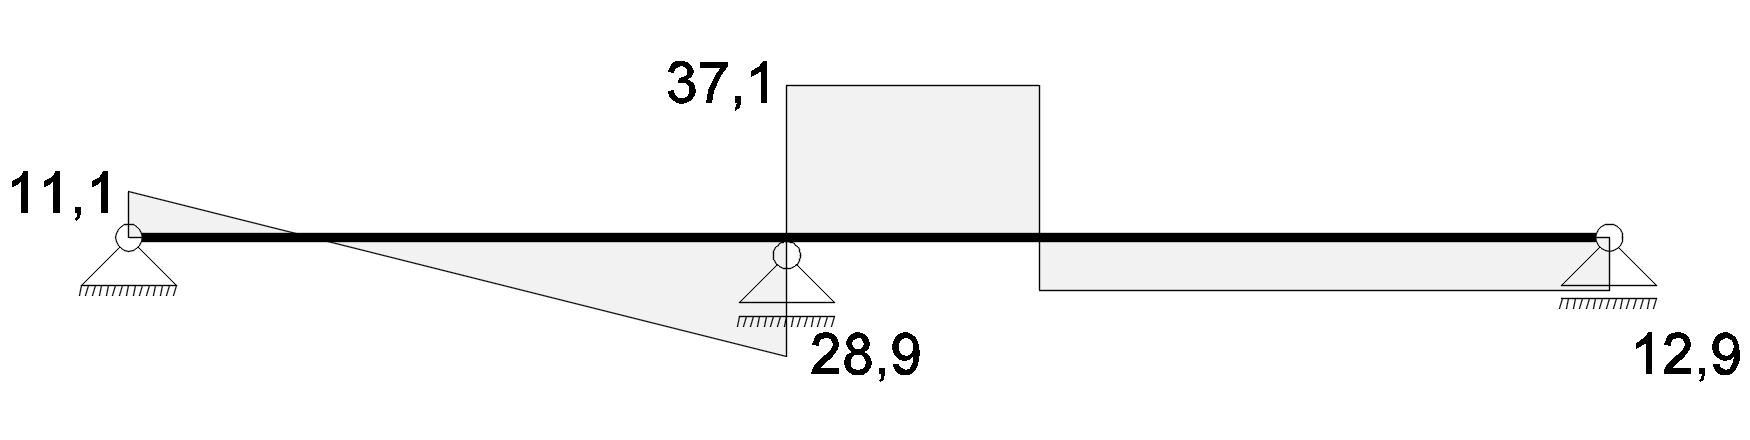
\includegraphics[width=.85\textwidth]{ej31V}
\end{center}

Diagrama de momentos (kN.m)

	\begin{center}
	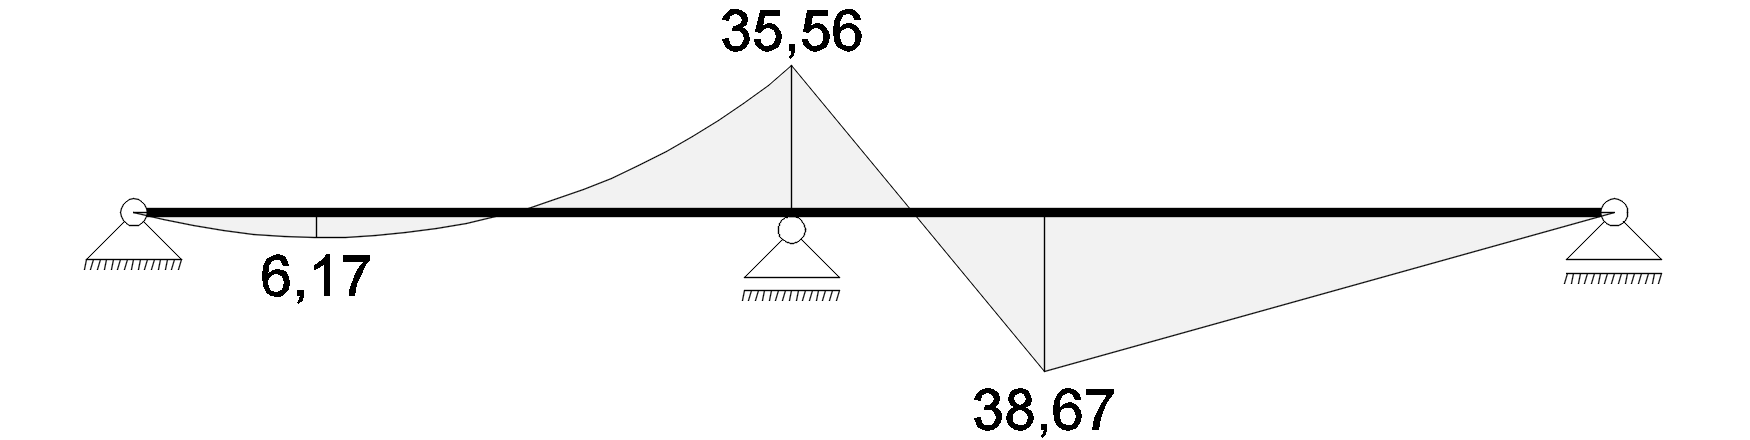
\includegraphics[width=.85\textwidth]{ej31M}
\end{center}

\item[3.2]
Mínima cantidad de incógnitas: 1 $\theta_B = 3.60 \times 10^{-3}$ rad.

Diagrama de directas (kN)

	\begin{center}
	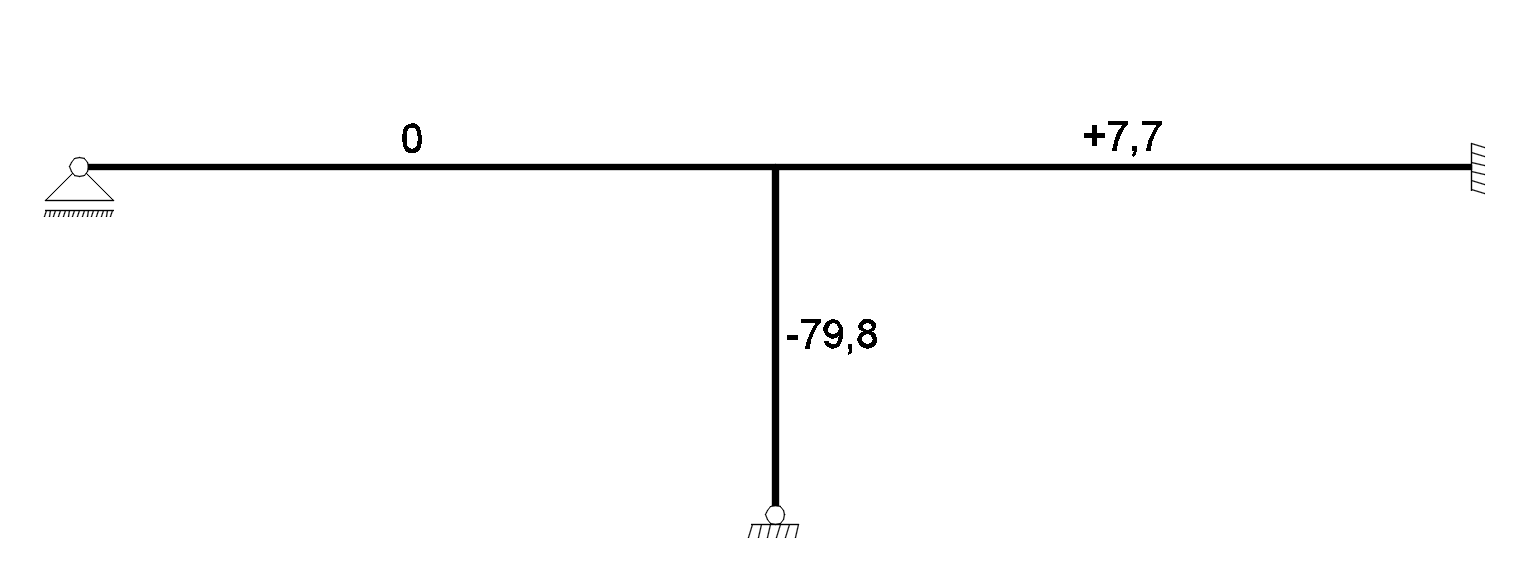
\includegraphics[width=.85\textwidth]{ej32N}
\end{center}

Diagrama de cortantes (kN)

	\begin{center}
	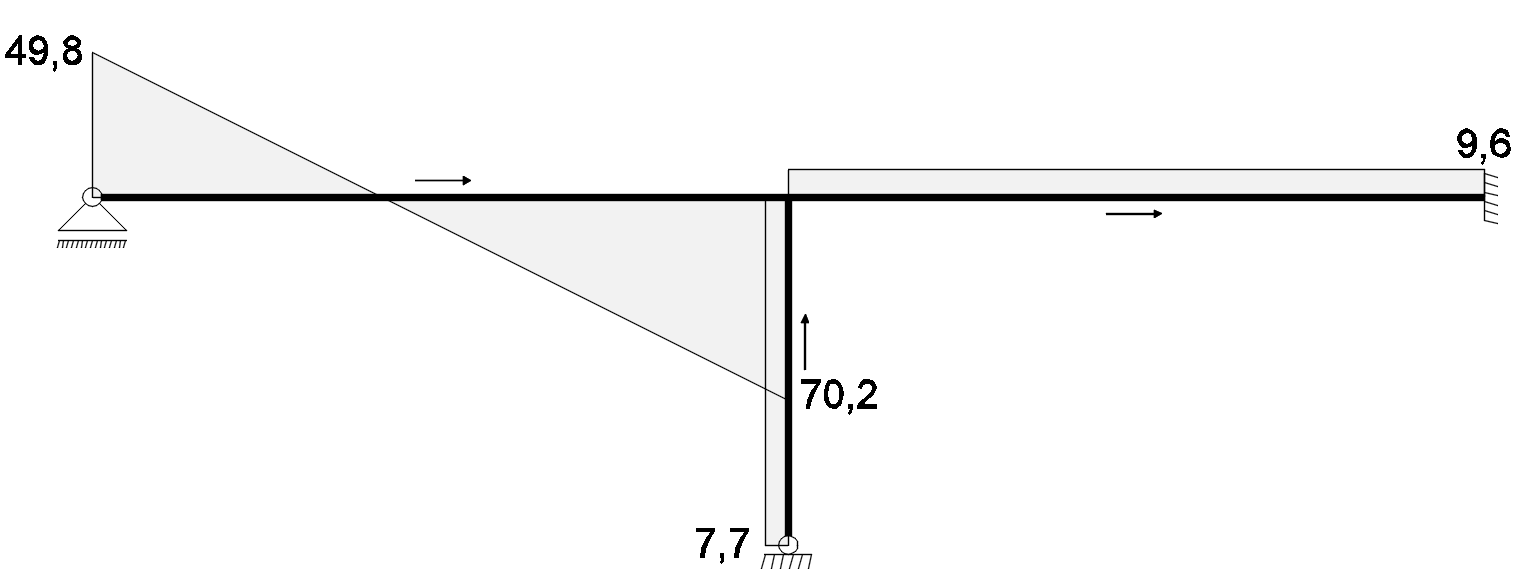
\includegraphics[width=.85\textwidth]{ej32V}
\end{center}

Diagrama de momentos (kN.m)

	\begin{center}
	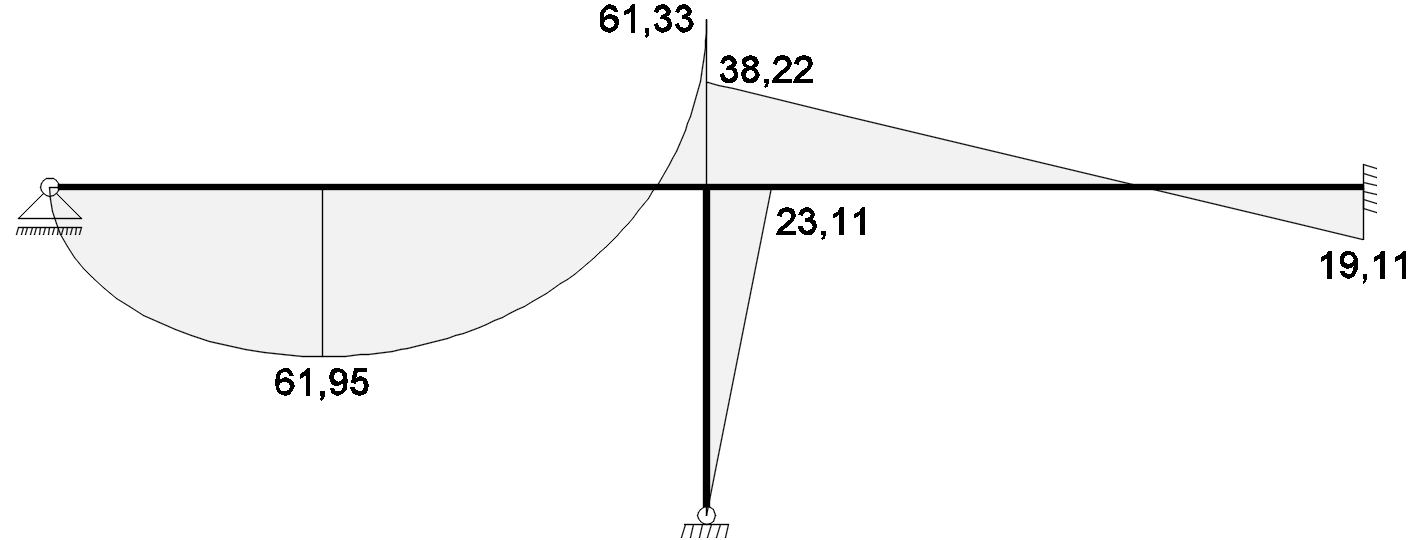
\includegraphics[width=.85\textwidth]{ej32M}
\end{center}

\item [3.3]

Mínima cantidad de incógnitas: 2, $\theta_A = -2.70 \times 10^{-3}$ rad y $\theta_B = 2.69 \times 10^{-3}$ rad.

$\mcN$ (kN)

	\begin{center}
	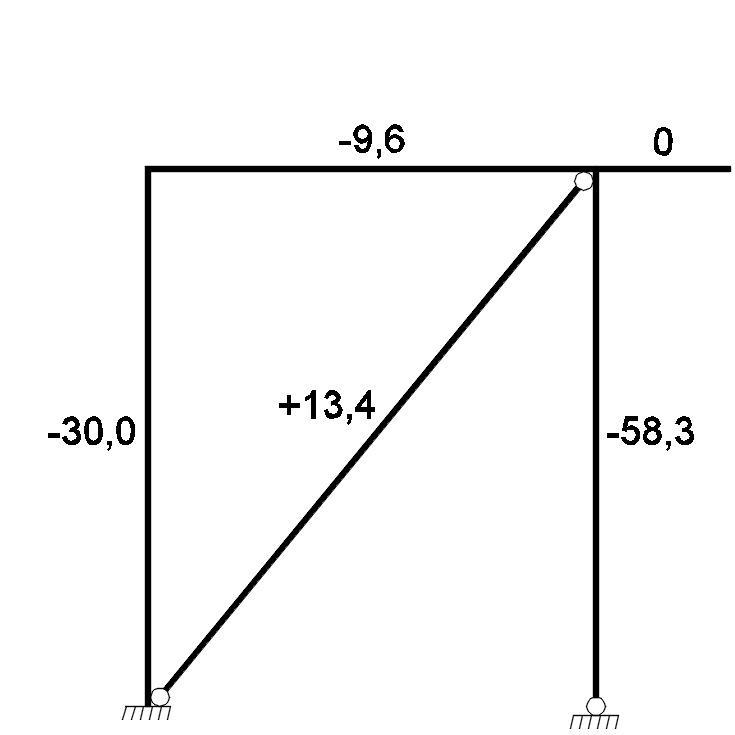
\includegraphics[width=.5\textwidth]{ej33N}
\end{center}

$\mcV$ (kN)

	\begin{center}
	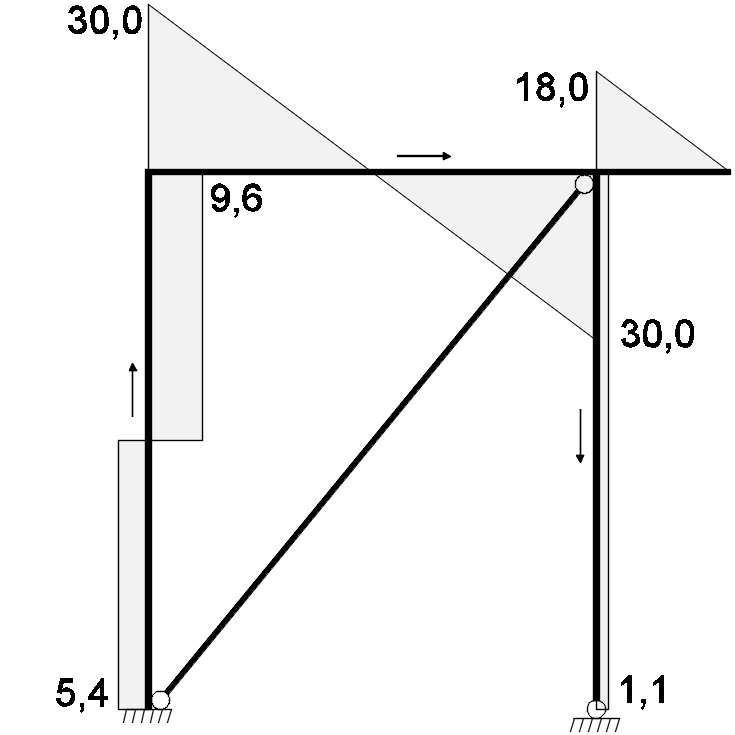
\includegraphics[width=.5\textwidth]{ej33V}
\end{center}

$\mcM$ (kNm)

	\begin{center}
	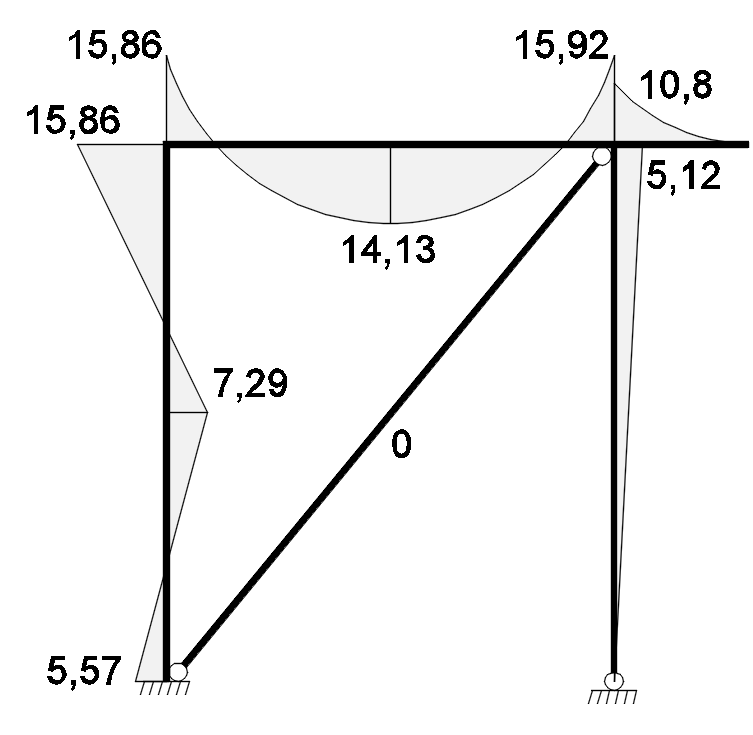
\includegraphics[width=.5\textwidth]{ej33M}
\end{center}

\item[3.4]
Mínima cantidad de incógnitas: 3, $\theta_B = -1.66 \times 10^{-3}$ rad, $\theta_C = 1.37 \times 10^{-3}$ rad y $\Delta = 6.75 \times 10^{-3}$ m (hacia la derecha).


$\mcN$ (kN)

\begin{center}
	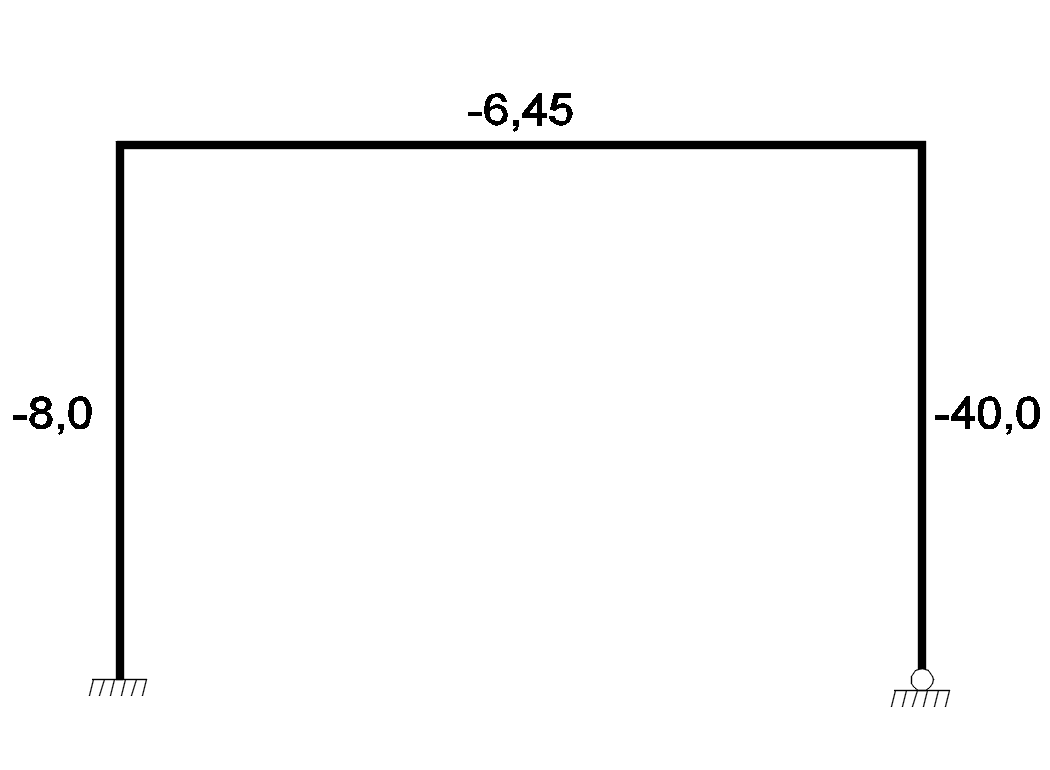
\includegraphics[width=.65\textwidth]{ej34N}
\end{center}

$\mcV$ (kN)

\begin{center}
	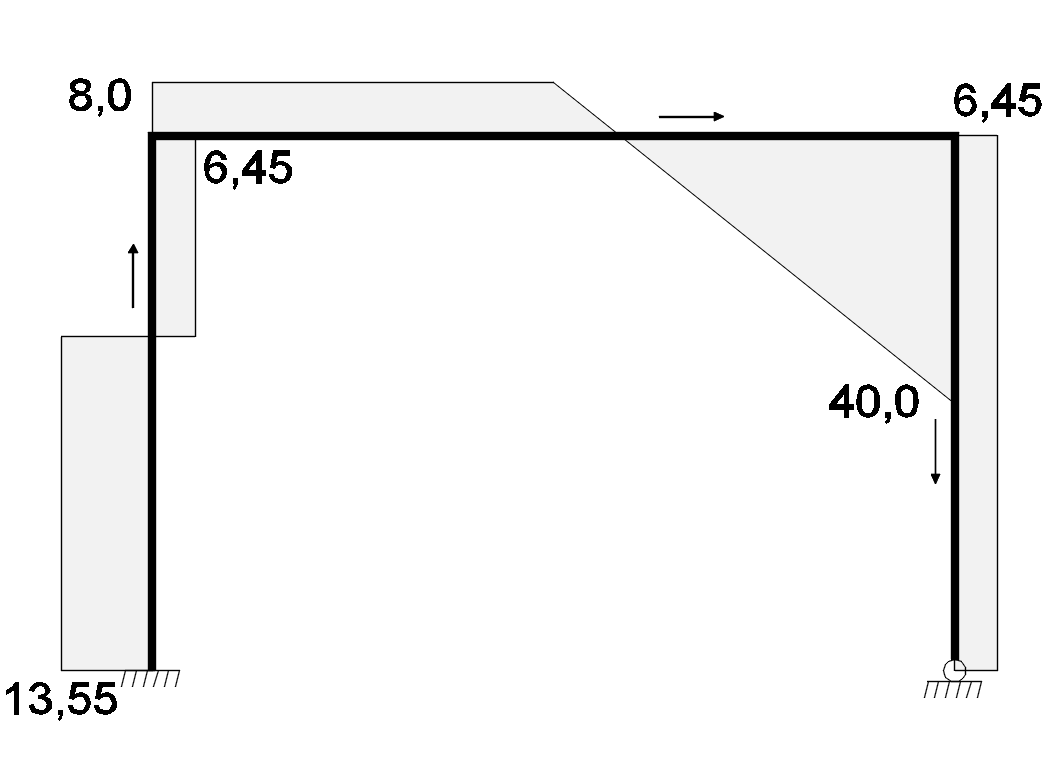
\includegraphics[width=.65\textwidth]{ej34V}
\end{center}

$\mcM$ (kNm)

\begin{center}
	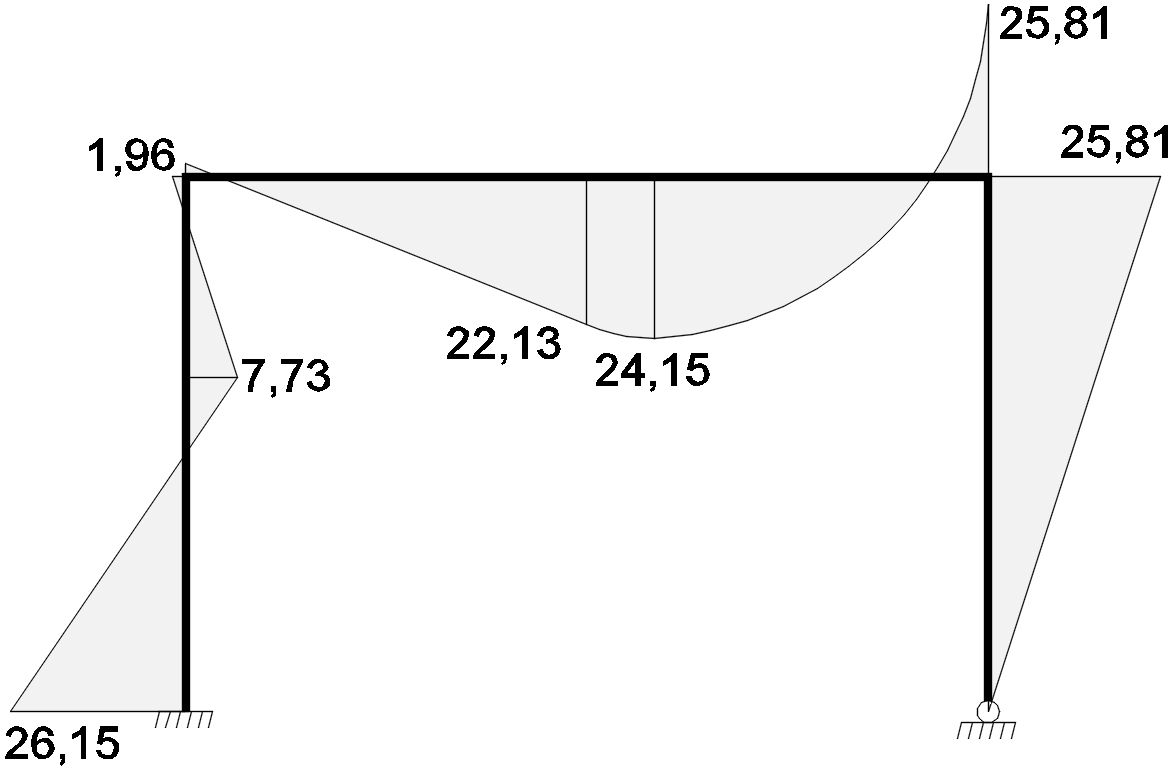
\includegraphics[width=.65\textwidth]{ej34M}
\end{center}


\item [3.5]

Mínima cantidad de incógnitas: 3, $\theta_C = -2.99 \times 10^{-3}$ rad, $ \theta_D = 3.04 \times 10^{-3}$ rad y $\Delta  = 14.42 \times 10^{-3}$ m (hacia la derecha).
%

$\mcN$ (kN)

\begin{center}
	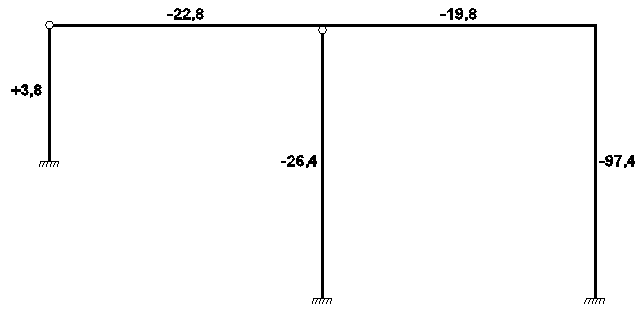
\includegraphics[width=.85\textwidth]{ej35N}
\end{center}

$\mcV$ (kN)

\begin{center}
	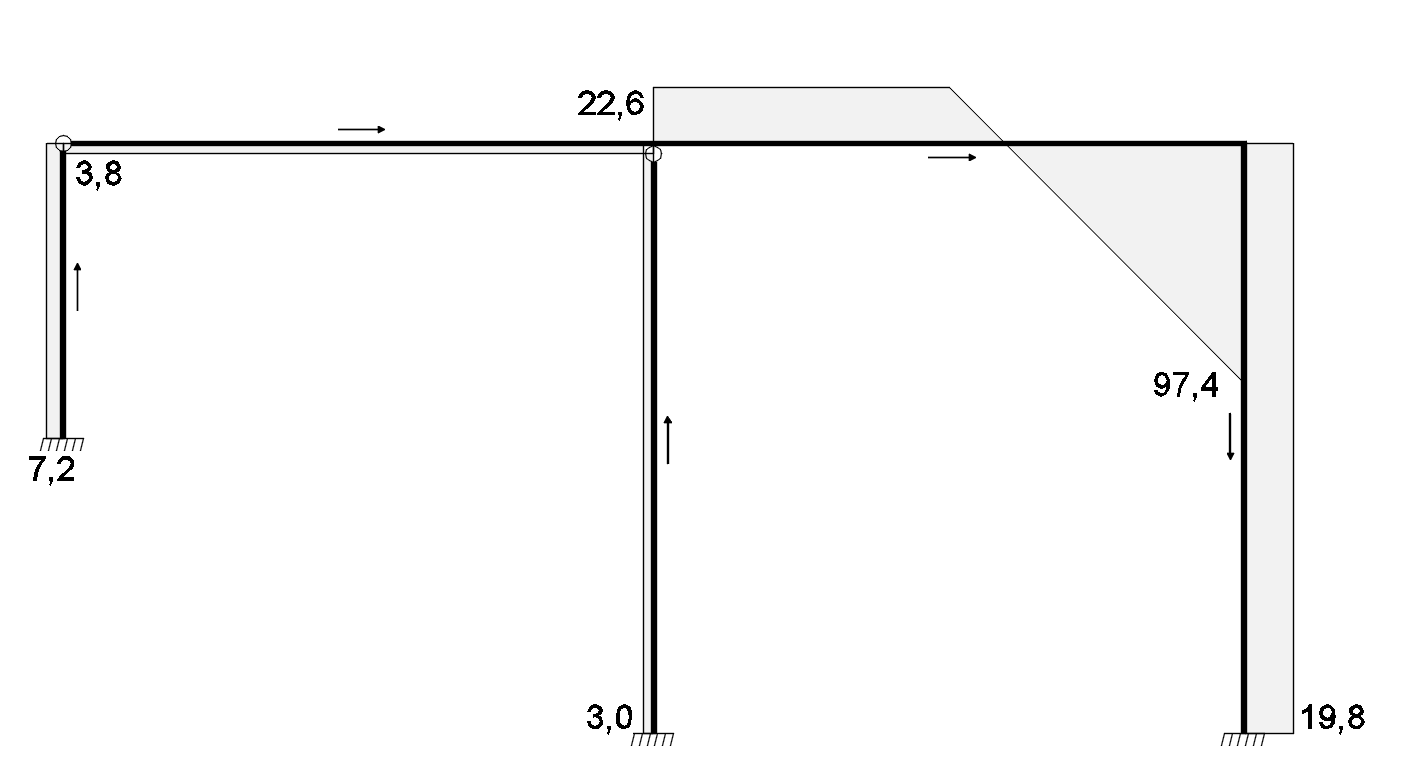
\includegraphics[width=.85\textwidth]{ej35V}
\end{center}

$\mcM$ (kNm)

\begin{center}
	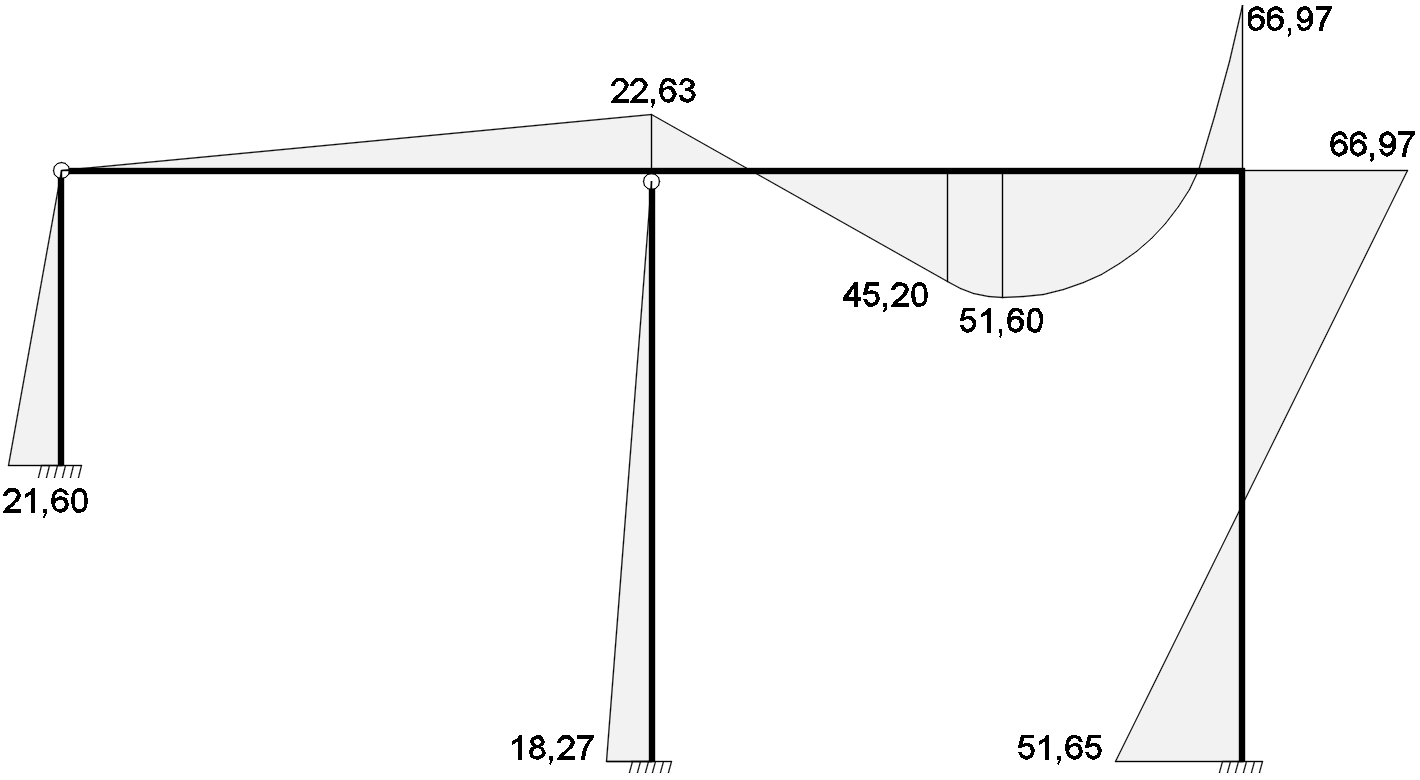
\includegraphics[width=.85\textwidth]{ej35M}
\end{center}



\item[3.6]
Mínima cantidad de incógnitas: 3, $\theta_B = 8.57 \times 10^{-4}$ rad, $\theta_C = 3.91 \times 10^{-4}$ rad y $\Delta  = 4.62 \times 10^{-3} $ m (hacia abajo).

$\mcN$ (kN)

\begin{center}
	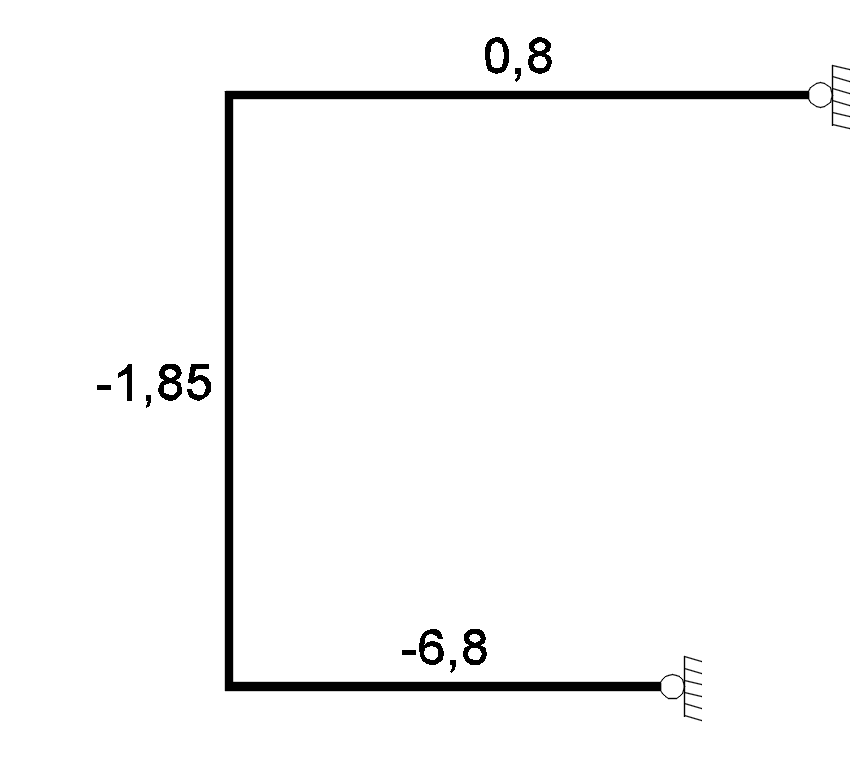
\includegraphics[width=.45\textwidth]{ej36N}
\end{center}

$\mcV$ (kN)

\begin{center}
	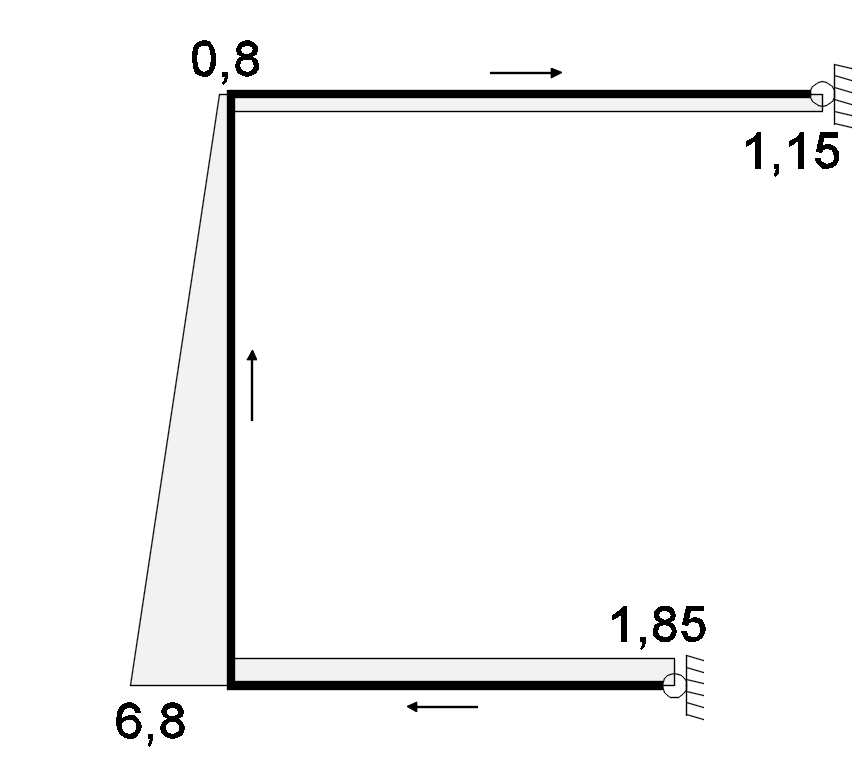
\includegraphics[width=.45\textwidth]{ej36V}
\end{center}

$\mcM$ (kNm)

\begin{center}
	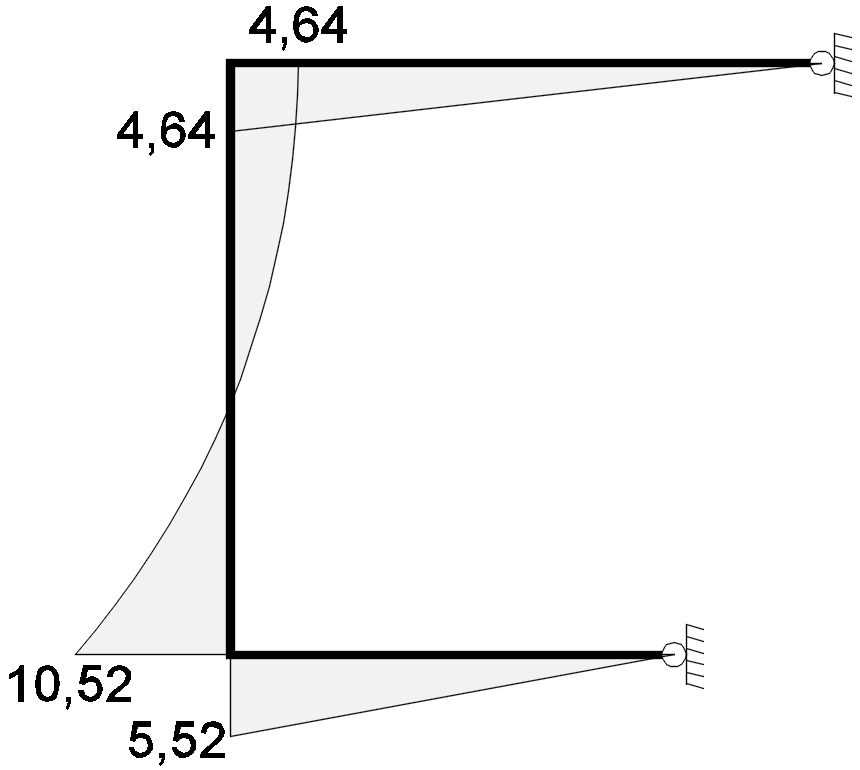
\includegraphics[width=.45\textwidth]{ej36M}
\end{center}

\item[3.7]

$a)$

\begin{center}
	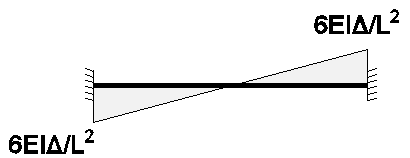
\includegraphics[width=.45\textwidth]{3.7a}
\end{center}

$b)$

\begin{center}
	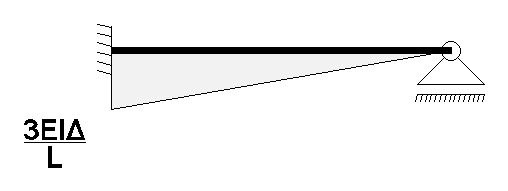
\includegraphics[width=.45\textwidth]{3.7b}
\end{center}

\end{description}

\section{Ejercicios de la UT4}

Las soluciones de los ejercicios están planteadas en base a la hipótesis de indeformabilidad de directa de aquellas barras que presentan flexión. Dicha hipótesis deberá ser corroborada para los distintos casos.


\begin{description}

\item[4.1] 

$\mcN$ (kN)
\begin{center}
	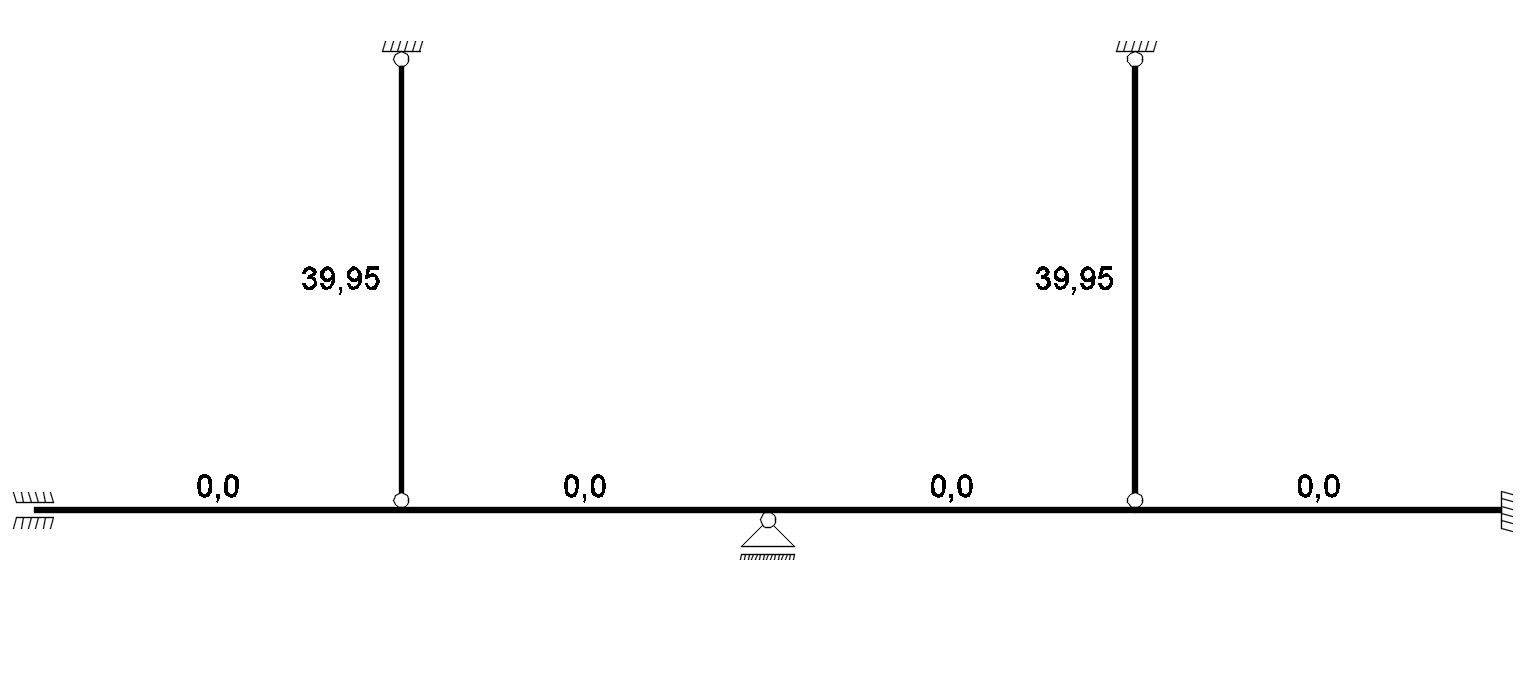
\includegraphics[width=.95\textwidth]{ej41N}
\end{center}


$\mcV$ (kN)
\begin{center}
	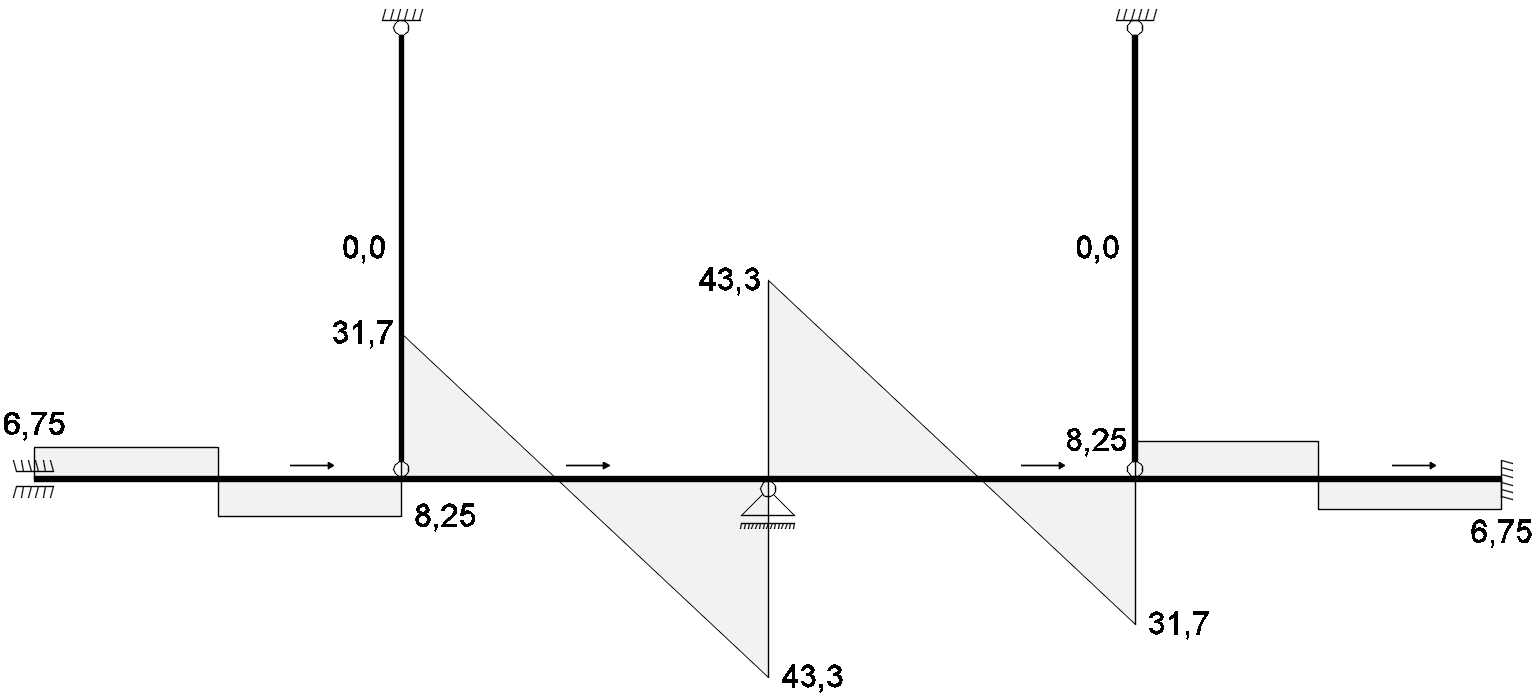
\includegraphics[width=.95\textwidth]{ej41V}
\end{center}

$\mcM$ (kN.m)
\begin{center}
	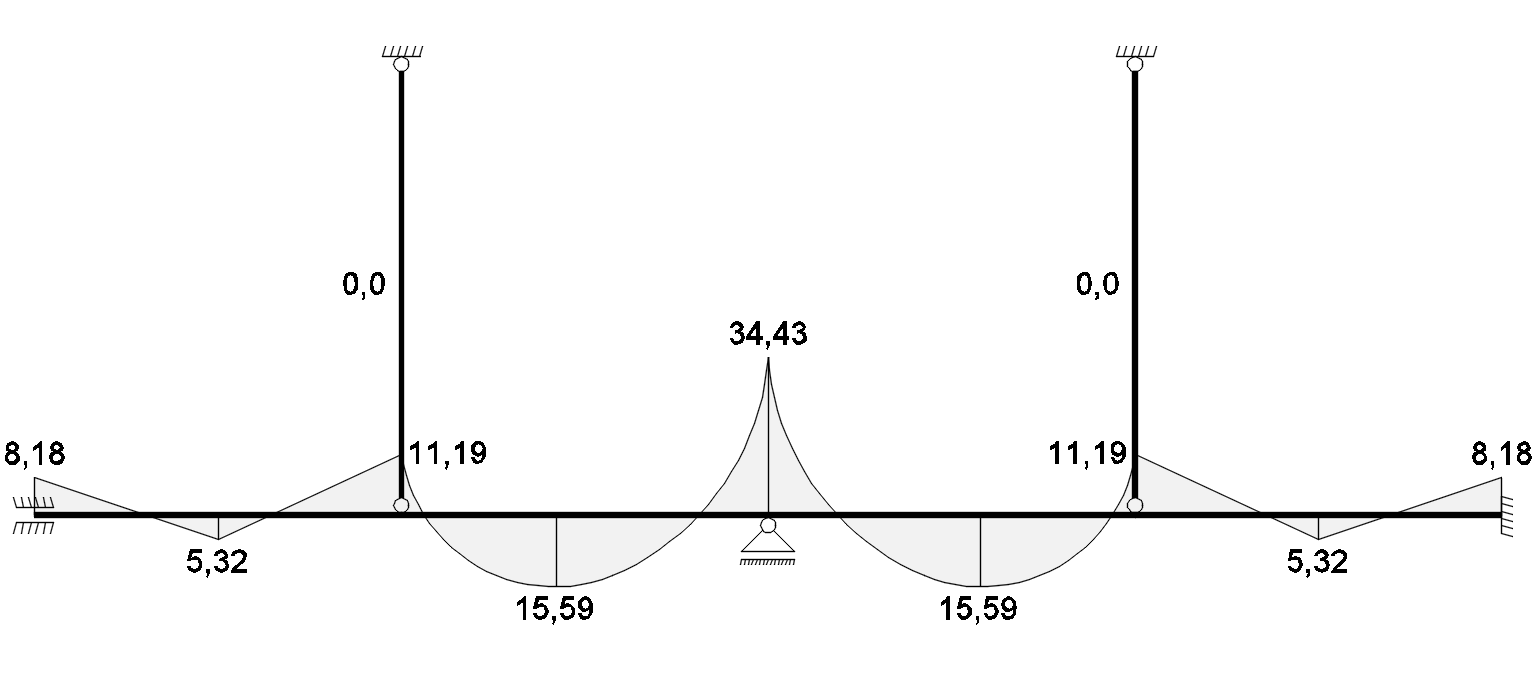
\includegraphics[width=.95\textwidth]{ej41M}
\end{center}


Deformada
\begin{center}
	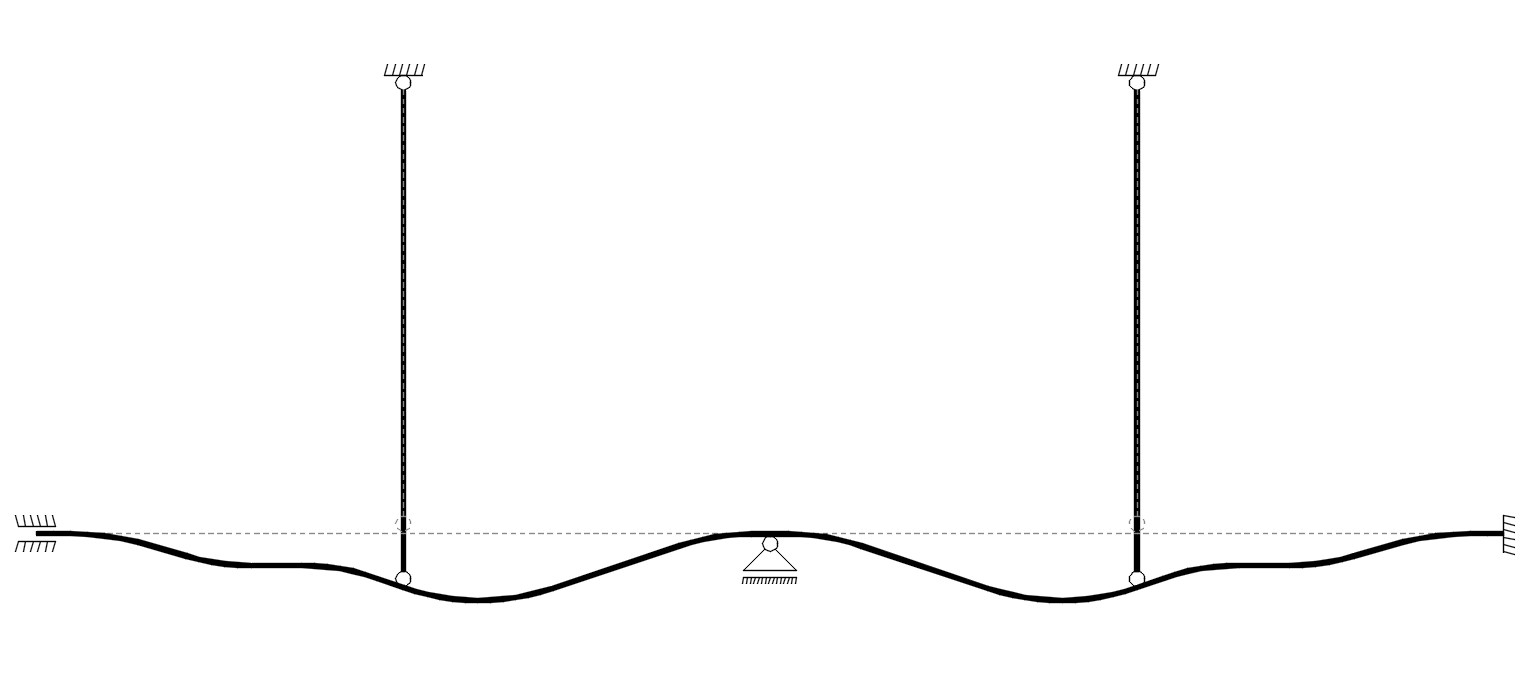
\includegraphics[width=.95\textwidth]{ej41def}
\end{center}



\item[4.2] 
\qquad \qquad
$\mcN$ (kN) \hspace{0.5\textwidth} $\mcV$ (kN)
\begin{center}
	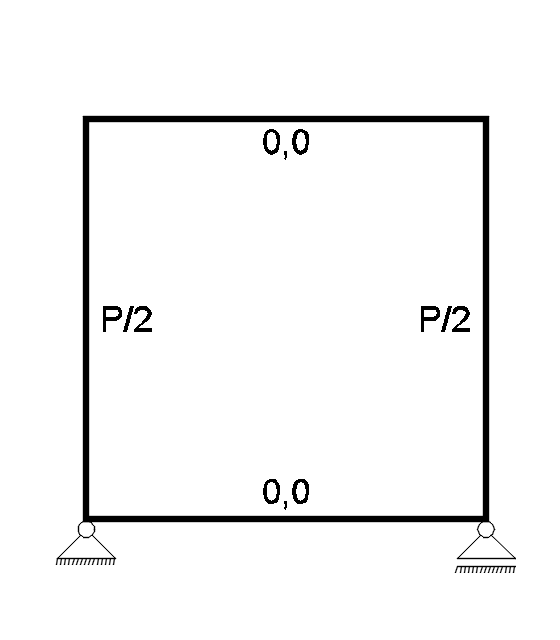
\includegraphics[width=.45\textwidth]{ej42N}
	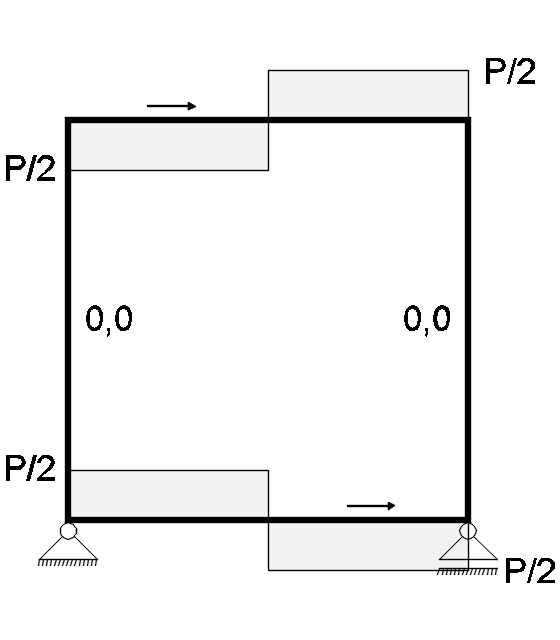
\includegraphics[width=.45\textwidth]{ej42V}
\end{center}

\qquad \qquad
$\mcM$ (kN.m)  \hspace{0.5\textwidth} Deformada
\begin{center}
	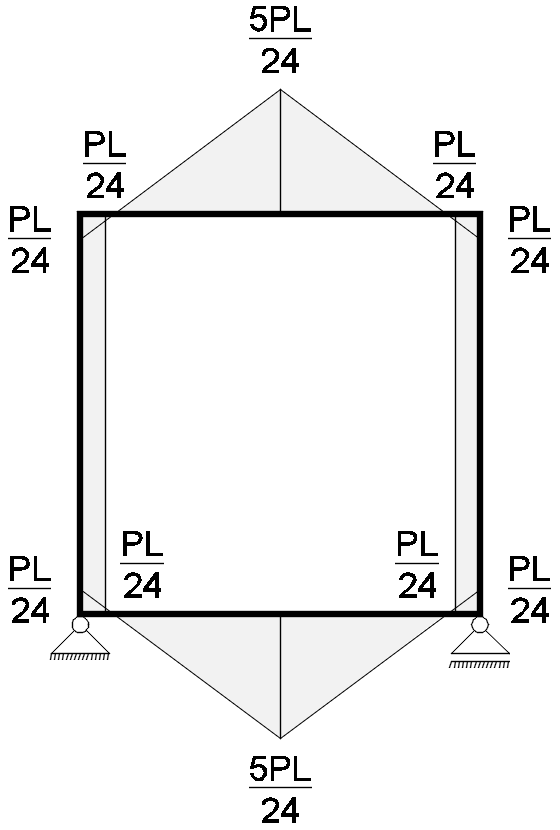
\includegraphics[width=.45\textwidth]{ej42M}
	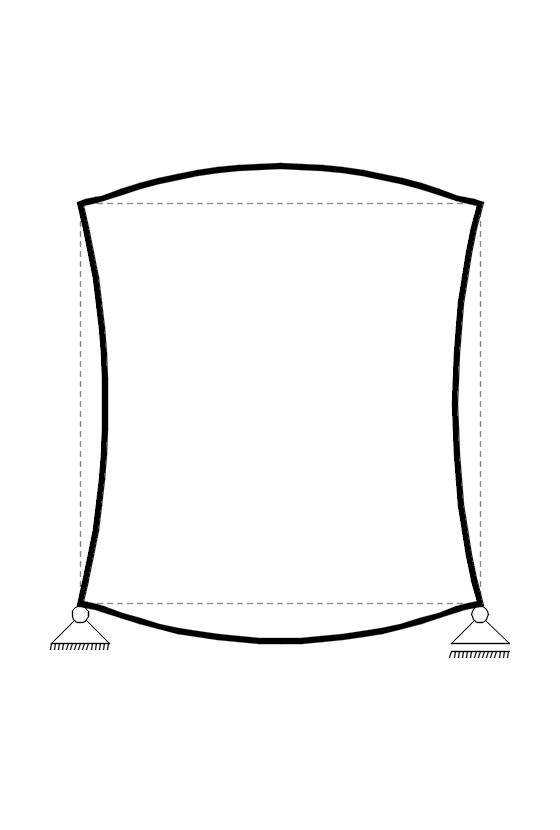
\includegraphics[width=.45\textwidth]{ej42def}
\end{center}


\item[4.3] 

$\mcN$ (kN) \hspace{0.4\textwidth} $\mcV$ (kN)
\begin{center}
	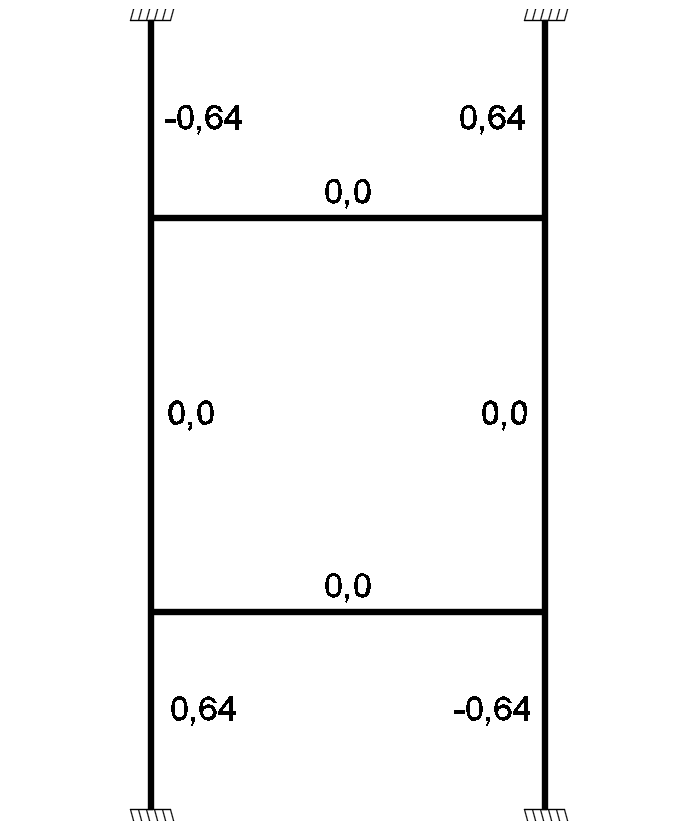
\includegraphics[width=.45\textwidth]{ej43N}
	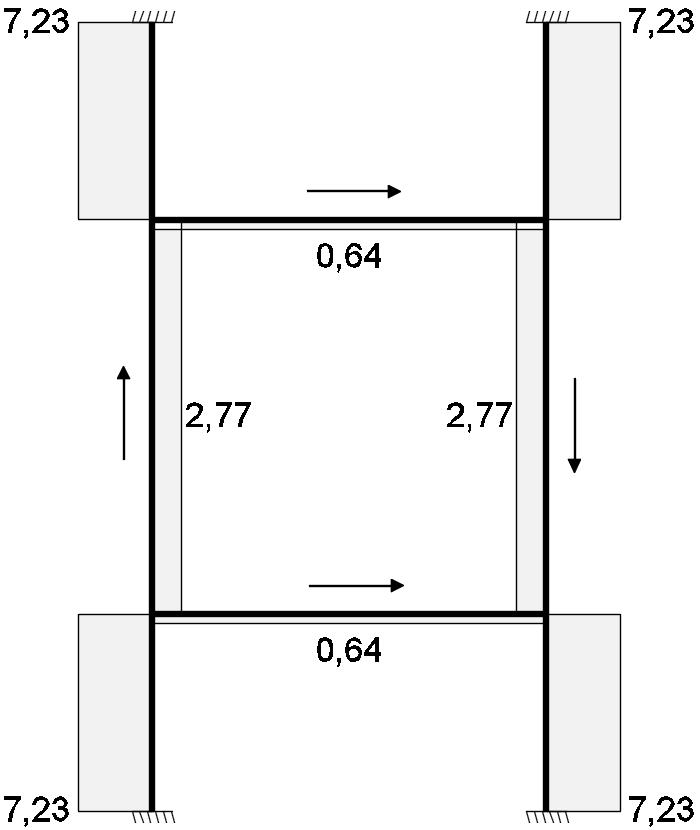
\includegraphics[width=.45\textwidth]{ej43V}
\end{center}

$\mcM$ (kN.m) \hspace{0.4\textwidth} Deformada
\begin{center}
	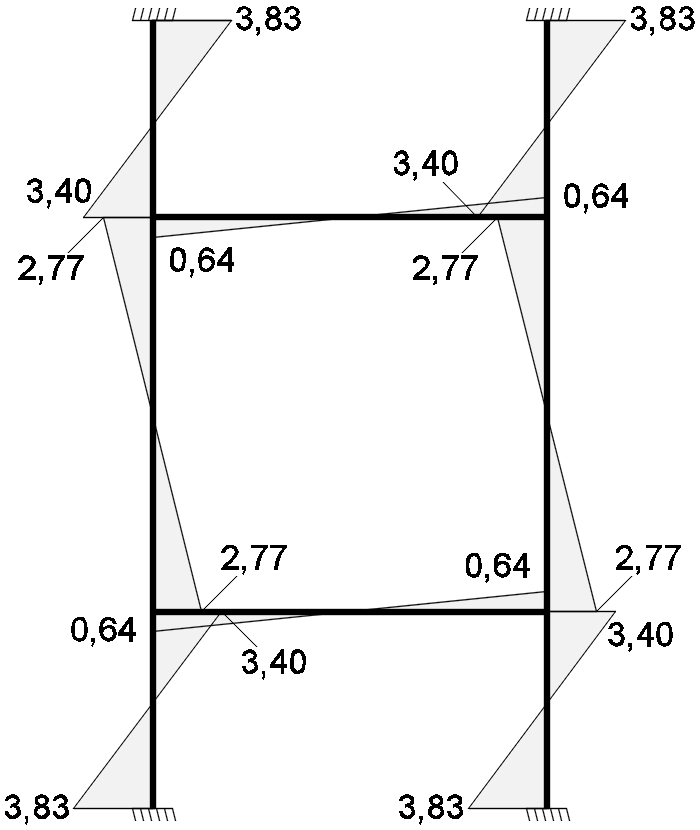
\includegraphics[width=.45\textwidth]{ej43M}
	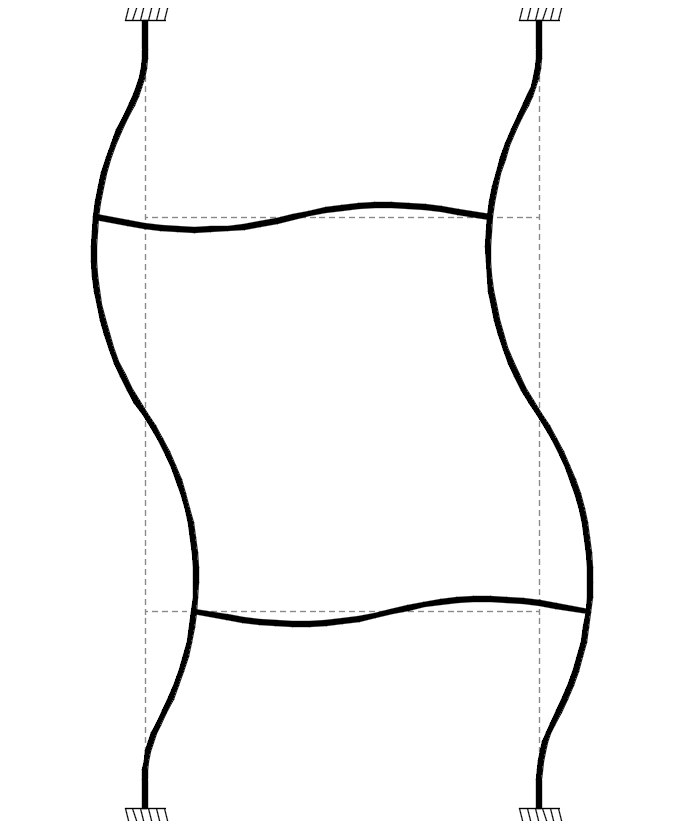
\includegraphics[width=.45\textwidth]{ej43def}
\end{center}


Giro de los puntos C, D, E y F, $-2.98 \times 10^{-4}$ rad.


\item[4.4]

\textbf{a)} $P = 17.5$ kN

\textbf{b)}

Giro en C: $\theta_C = 5.6 \times 10^{-4}$ rad.

Giro en D: $\theta_D = -5.6 \times 10^{-4}$ rad.

Desplazamiento de M: $\Delta_M = 2.99 \times 10^{-3}$ m (hacia abajo).

\item [4.5]
\textbf{a)} $\alpha_1 = 0.457$ , $\alpha_2 = 0.163$ , $\alpha_3 = -0.120$.

$\mcN$ (kN) \hspace{0.4\textwidth} $\mcV$ (kN)

\begin{center}
	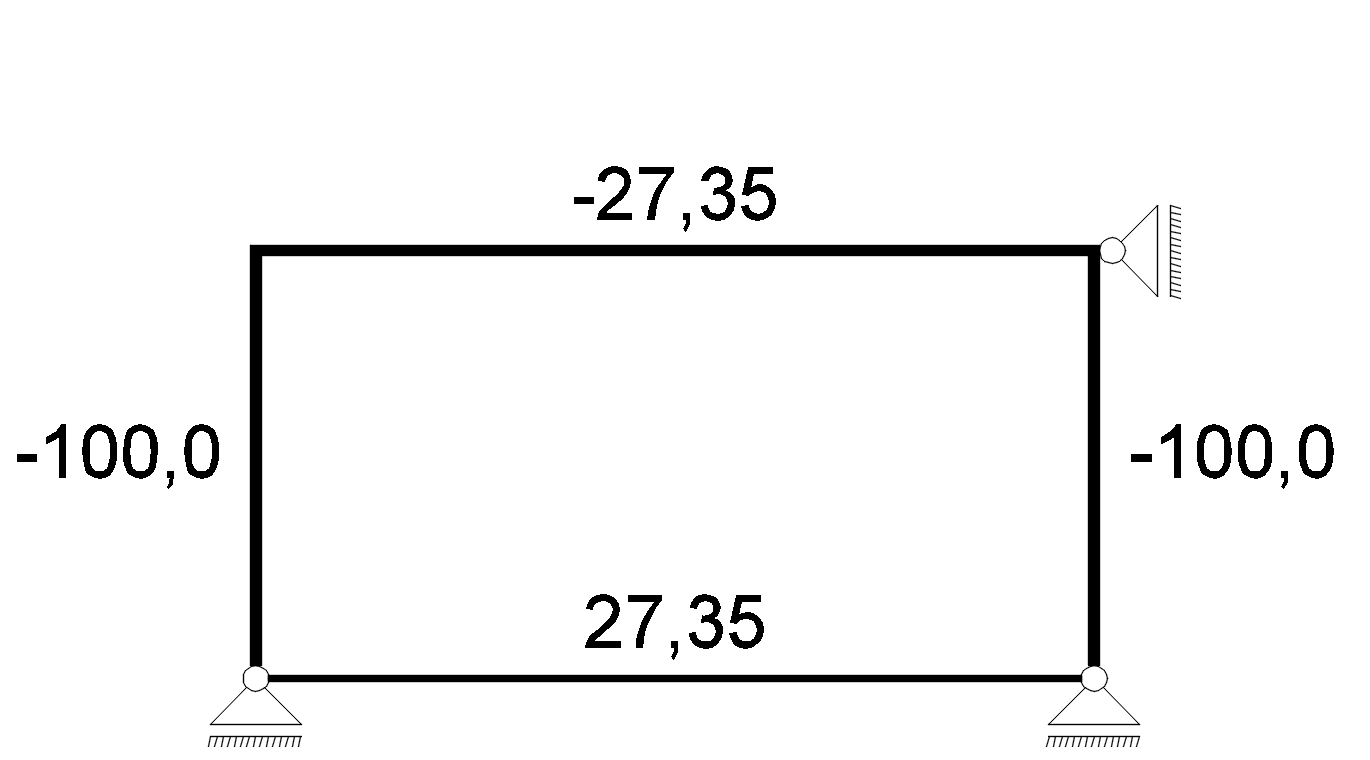
\includegraphics[width=.45\textwidth]{ej45N}
	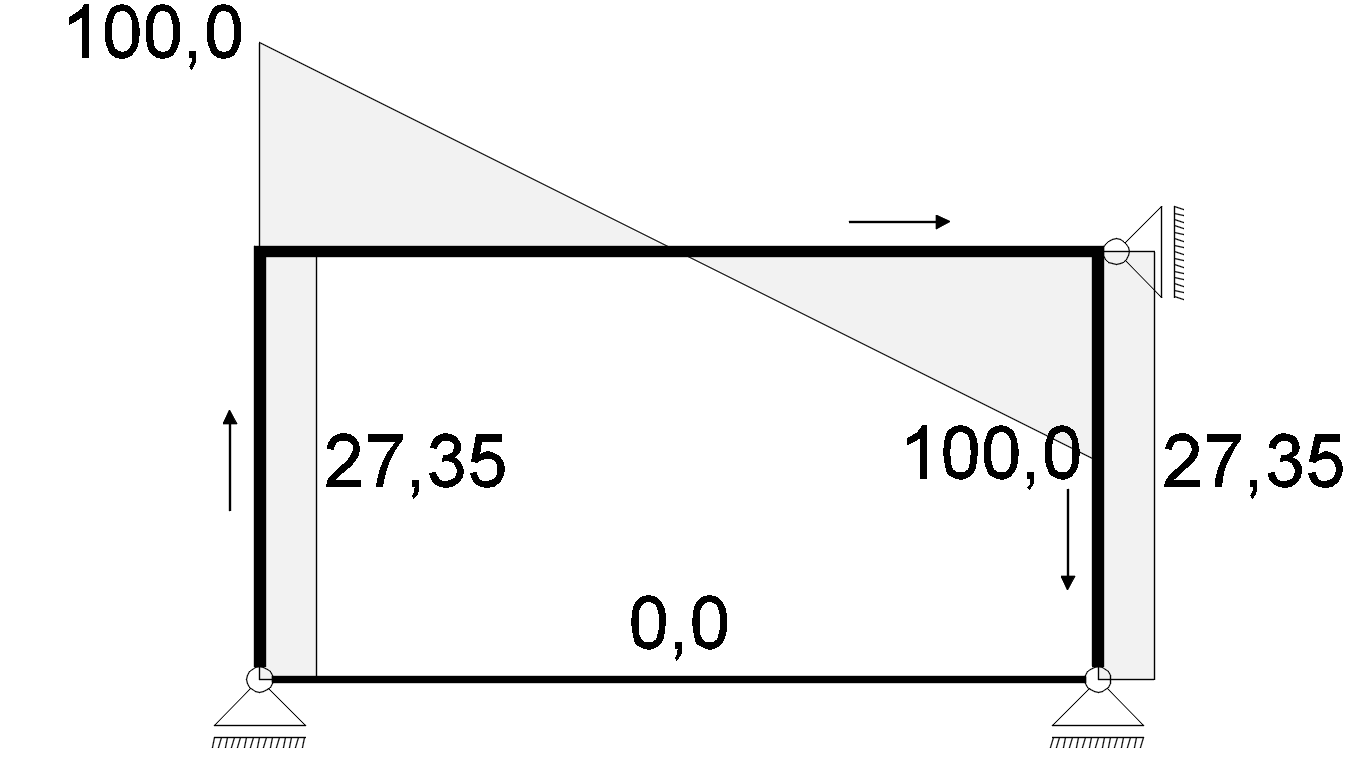
\includegraphics[width=.45\textwidth]{ej45V}
\end{center}

$\mcM$ (kN.m)

\begin{center}
	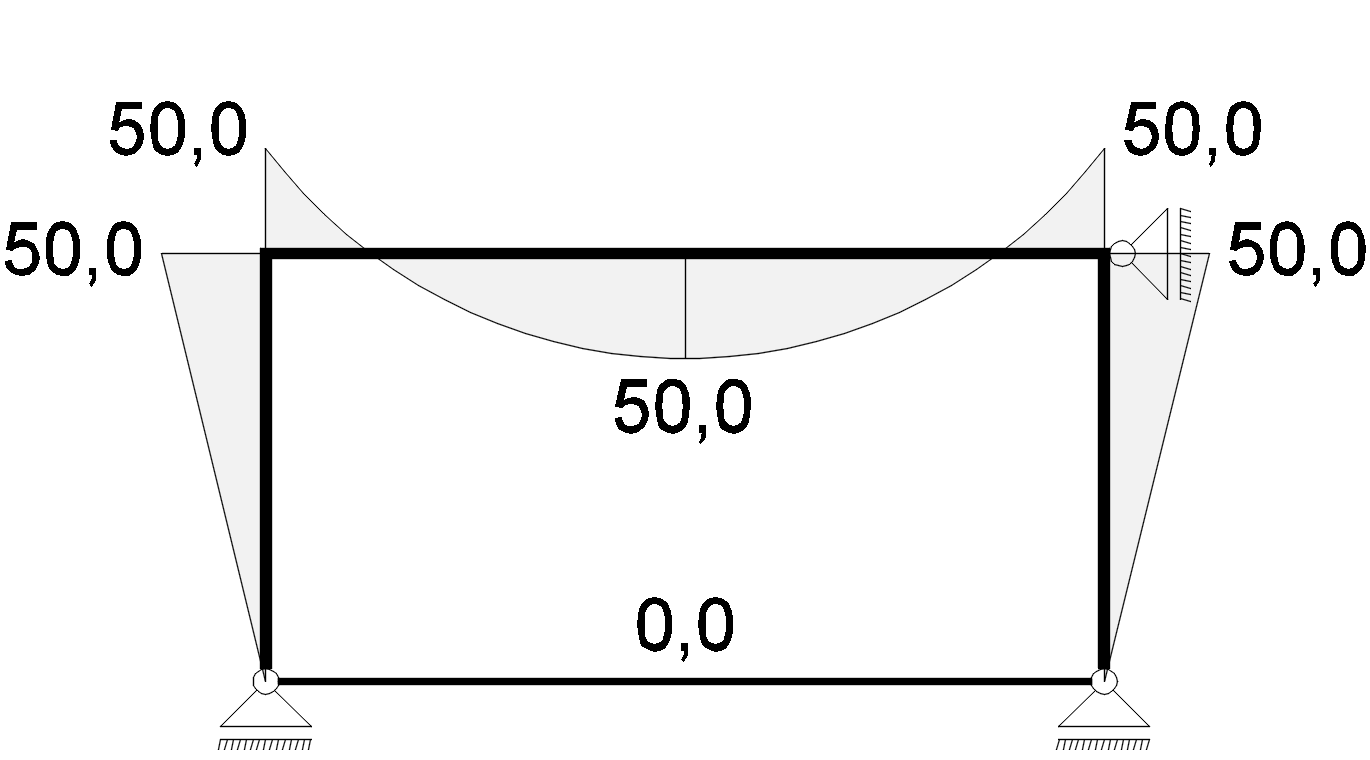
\includegraphics[width=.45\textwidth]{ej45M}
\end{center}


\item[4.6]

\textbf{a)} $t = 2.5$ cm

\textbf{b)} $k = 2000$ kN/m


$\mcN$ (kN)
\begin{center}
	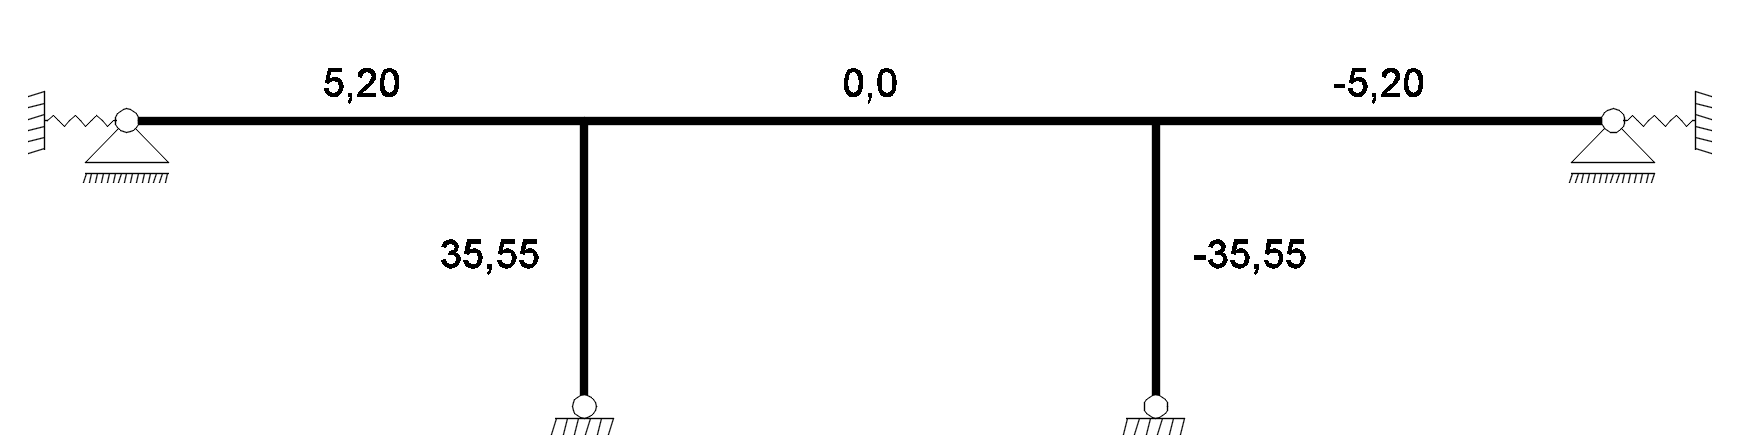
\includegraphics[width=.95\textwidth]{ej46N}
\end{center}

$\mcV$ (kN)
\begin{center}
	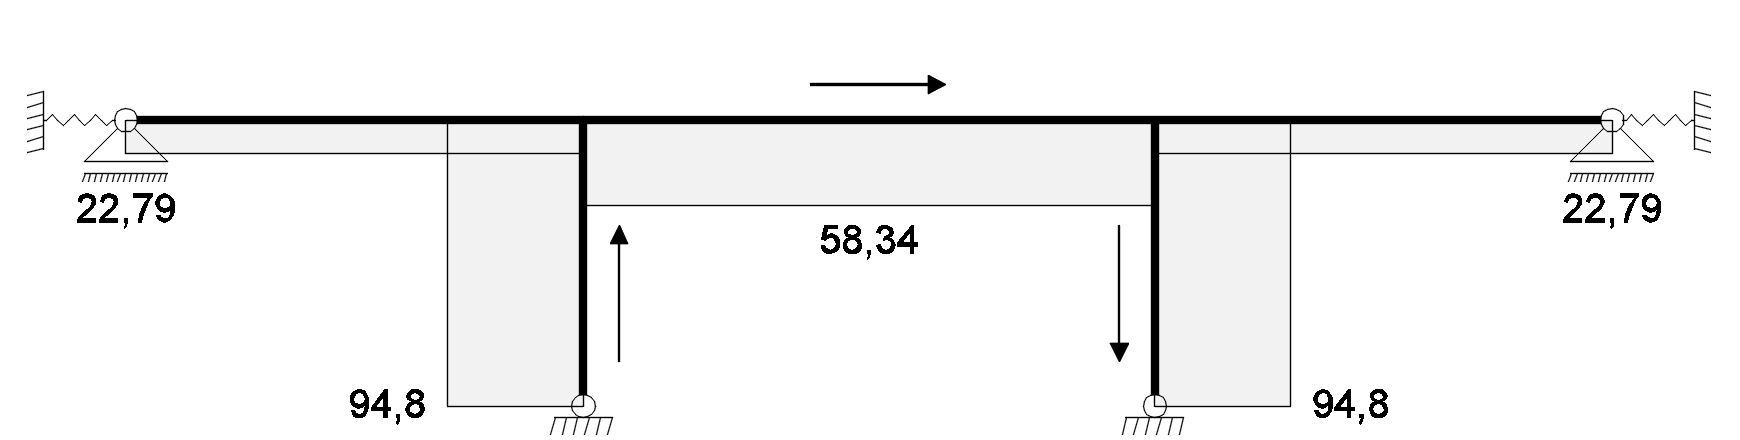
\includegraphics[width=.95\textwidth]{ej46V}
\end{center}

$\mcM$ (kNmm)

\begin{center}
	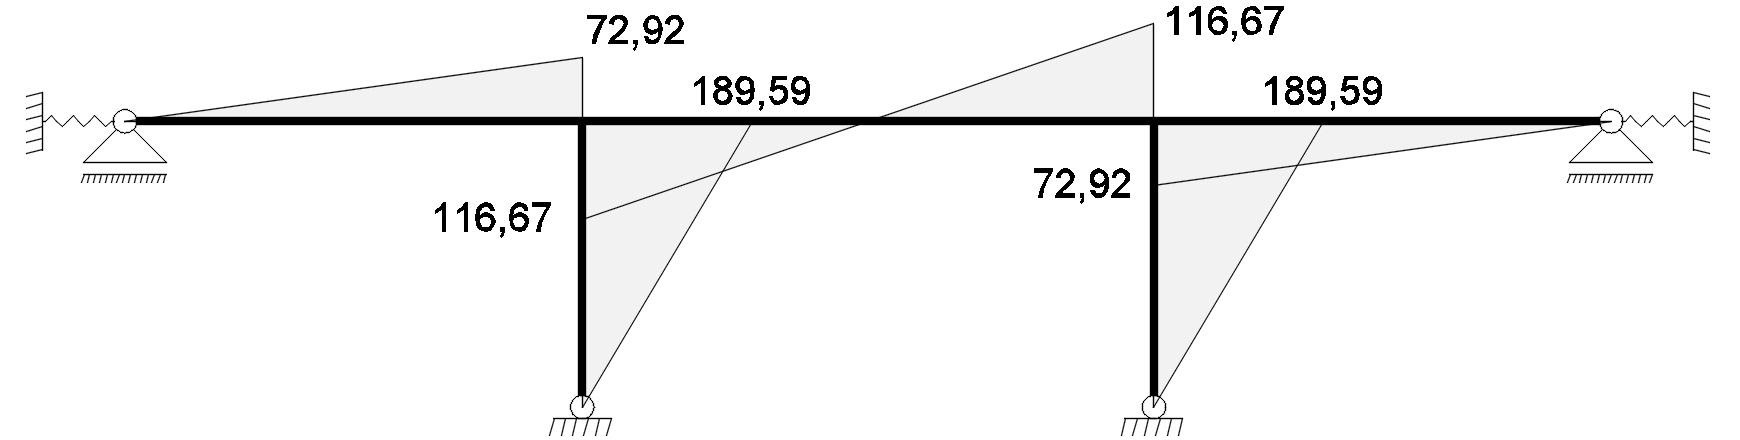
\includegraphics[width=.95\textwidth]{ej46M}
\end{center}


Deformada

\begin{center}
	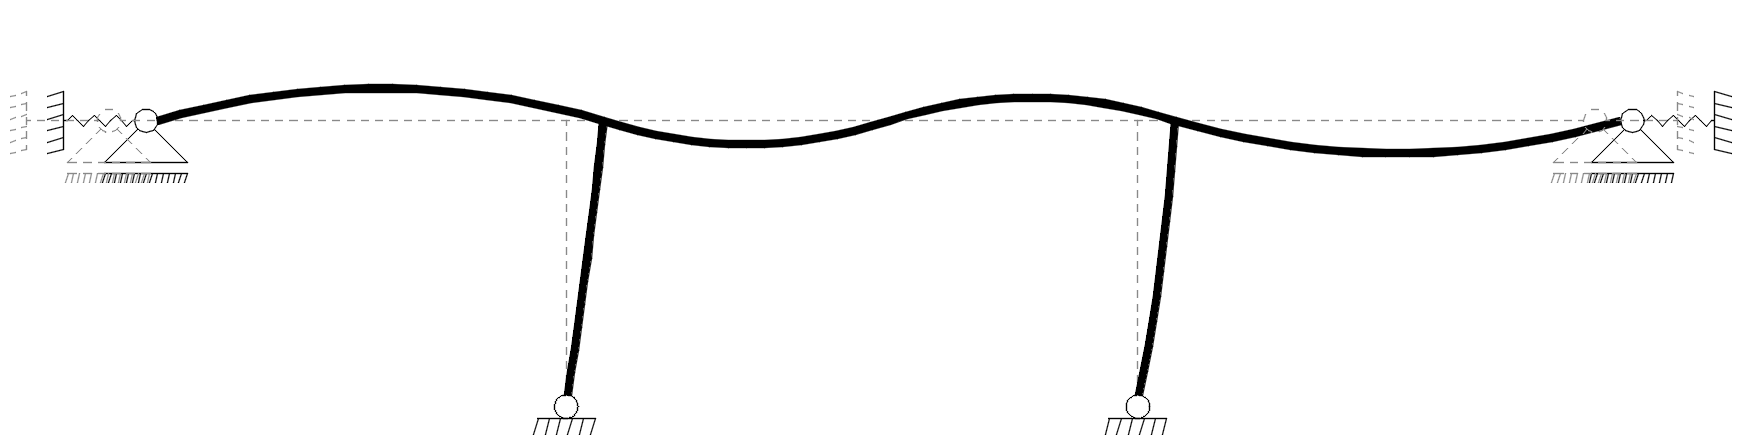
\includegraphics[width=.95\textwidth]{ej46def}
\end{center}


\item[4.7]

\textbf{a)} $k = 1200$ kN/m

\textbf{b)} $a = 2.82$ m

\textbf{c)} $\sigma_{max} = 6.85$  MPa

$\mcN$ (kN)

\begin{center}
	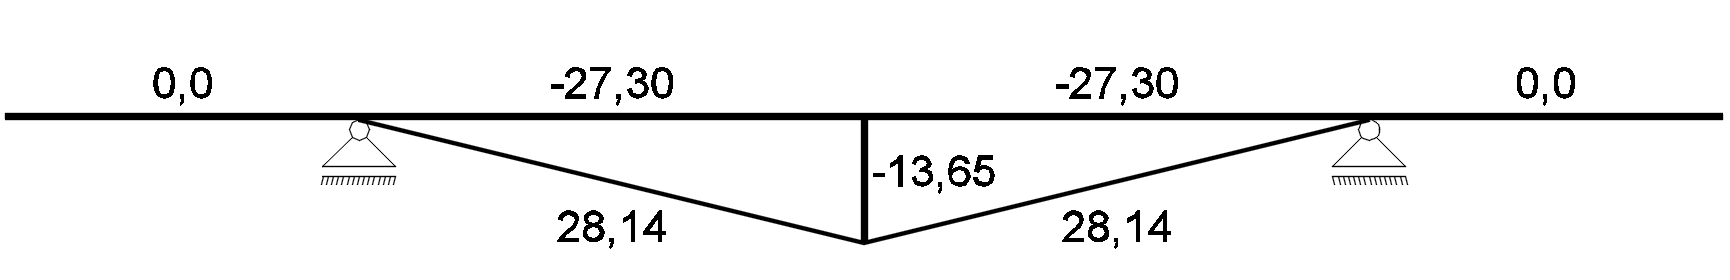
\includegraphics[width=.95\textwidth]{ej47N}
\end{center}

$\mcV$ (kN)

\begin{center}
	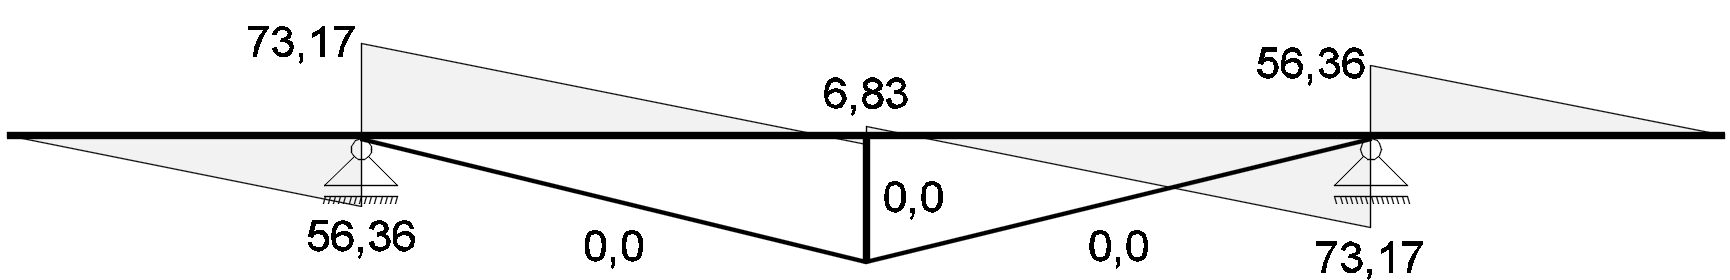
\includegraphics[width=.95\textwidth]{ej47V}
\end{center}

$\mcM$ (kN.m)

\begin{center}
	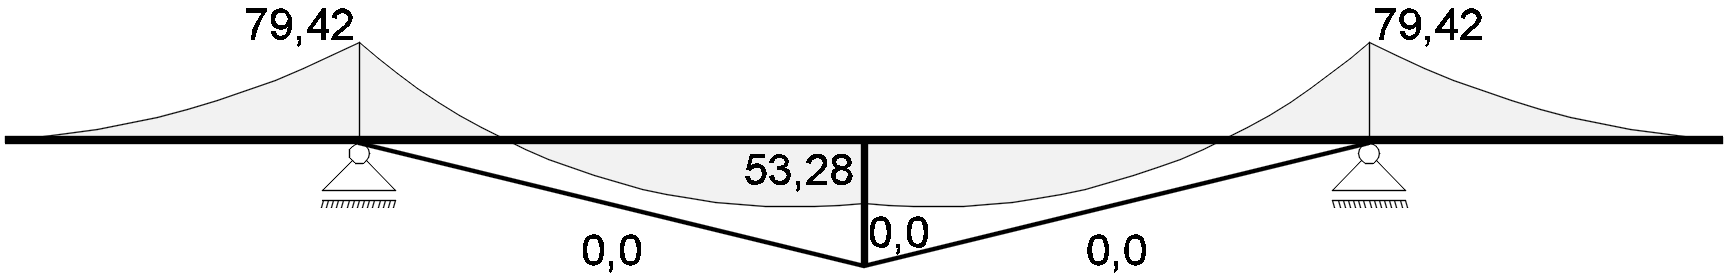
\includegraphics[width=.95\textwidth]{ej47M}
\end{center}

\item[4.8]
\textbf{a)}

Giro en C: $\theta_C = 3.16 \times 10^{-3}$.

Desplazamiento de C: $\Delta_C = 2.53 \times 10^{-2}$ m (hacia la izquierda).

$\mcN$ (kN) \hspace{0.4\textwidth} $\mcV$ (kN)
\begin{center}
	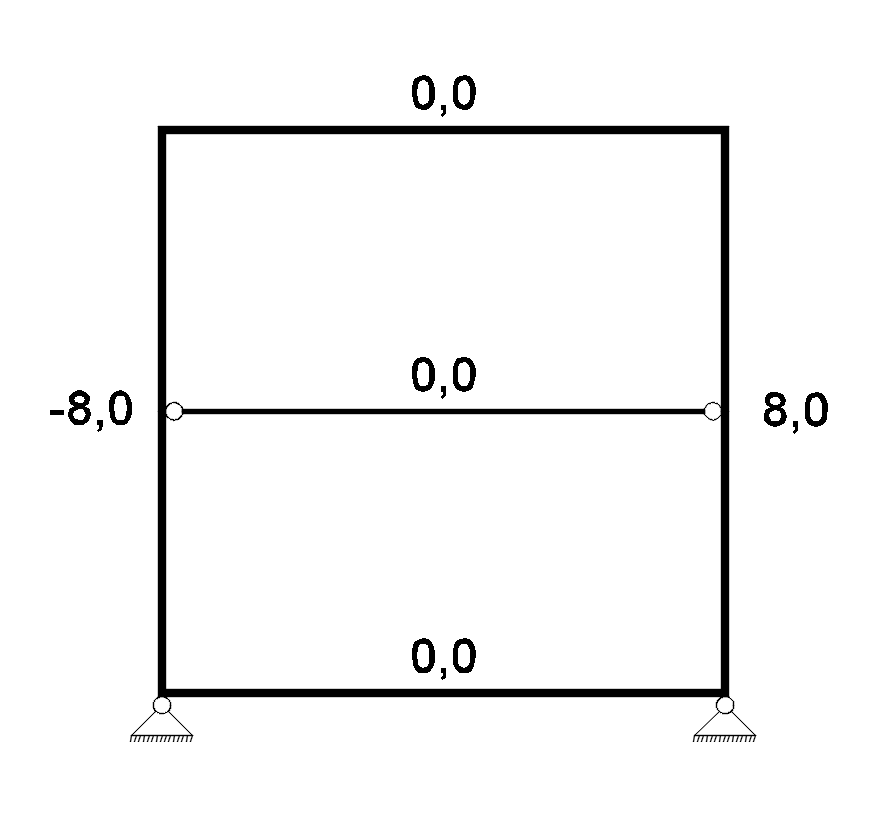
\includegraphics[width=.45\textwidth]{ej48N}
	\includegraphics[width=.45\textwidth]{ej48V}
\end{center}

$\mcM$ (kN.m) \hspace{0.4\textwidth} deformada
\begin{center}
	\includegraphics[width=.45\textwidth]{ej48M}
	\includegraphics[width=.45\textwidth]{ej48def}
\end{center}

\item [4.9]

$\mcN$ (kN) \hspace{0.4\textwidth} $\mcV$ (kN)
\begin{center}
	\includegraphics[width=.45\textwidth]{ej49N}
	\includegraphics[width=.45\textwidth]{ej49V}
\end{center}

$\mcM$ (kN.m) \hspace{0.4\textwidth} deformada
\begin{center}
	\includegraphics[width=.45\textwidth]{ej49M}
	\includegraphics[width=.45\textwidth]{ej49def}
\end{center}

\end{description}




\section{Ejercicios de la UT5}

\begin{description}

\item[5.1]

\begin{minipage}{0.45\textwidth}
	Sist. de coord
	
	\includegraphics[width=\textwidth]{ej51ejes}
\end{minipage}
~
\begin{minipage}{0.45\textwidth}
Incógnitas cinemáticas,
$$
\left[
\begin{matrix}
\theta_{x,2} \\
v_{y,2} \\
\theta_{z,2}
\end{matrix}
\right]
=
\left[
\begin{matrix}
-1.00\times 10^{-2} \text{ rad }\\
-2.56\times 10^{-3} \text{ m }\\
-3.86\times 10^{-3} \text{ rad }
\end{matrix}
\right]
$$

$$
\left[
\begin{matrix}
\theta_{x,3} \\
v_{y,3} \\
\theta_{z,3}
\end{matrix}
\right]
=
\left[
\begin{matrix}
-1.39\times 10^{-2} \text{ rad }\\
-1.52\times 10^{-2} \text{ m }\\
-3.86\times 10^{-3} \text{ rad }
\end{matrix}
\right]
$$
\end{minipage}

\vspace{5mm}

\begin{minipage}{0.45\textwidth}
Cortante - Vy,local (kN)

\includegraphics[width=\textwidth]{ej51Vy}
\end{minipage}
~
\begin{minipage}{0.45\textwidth}
Flexión - Mz,local (kN.m)

\includegraphics[width=\textwidth]{ej51Mz}
\end{minipage}


\begin{center}
Torsor - Mx,local (kN.m)

\includegraphics[width=.45\textwidth]{ej51Mx}
\end{center}




\hrule 

\item[5.2]


Estructura Figura 1.a

Sistema de coordenadas
\begin{center}
\includegraphics[width=.6\textwidth]{ej52ejes}
\end{center}


\begin{minipage}{0.45\textwidth}
	Incógnitas cinemáticas,
$$
\left[
\begin{matrix}
\theta_{x,2} \\
v_{y,2} \\
\theta_{z,2}
\end{matrix}
\right]
=
\left[
\begin{matrix}
-7.28\times 10^{-4} \text{ rad }\\
-1.29\times 10^{-3} \text{ m }\\
-1.93\times 10^{-3} \text{ rad }
\end{matrix}
\right]
$$

$$
\left[
\begin{matrix}
\theta_{x,3} \\
v_{y,3} \\
\theta_{z,3}
\end{matrix}
\right]
=
\left[
\begin{matrix}
 7.28\times 10^{-4} \text{ rad }\\
-1.29\times 10^{-3} \text{ m }\\
-1.93\times 10^{-3} \text{ rad }
\end{matrix}
\right]
$$
\end{minipage}
~
\begin{minipage}{0.45\textwidth}
Cortante $V_y$ (N)

\includegraphics[width=\textwidth]{ej52Vy}
\end{minipage}


Flexión - Mz,local (kN.m) \hfill  Torsor - Mx,local (kN.m)

\includegraphics[width=.45\textwidth]{ej52Mz}
\includegraphics[width=.45\textwidth]{ej52Mx}


\hrule 

Estructura Figura 1.b



\begin{minipage}{0.45\textwidth}
	Incógnitas cinemáticas,
	$$
	\left[
	\begin{matrix}
	\theta_{x,2} \\
	v_{y,2} \\
	\theta_{z,2}
	\end{matrix}
	\right]
	=
	\left[
	\begin{matrix}
	 1.91\times 10^{-4} \text{ rad }\\
	-4.01\times 10^{-4} \text{ m }\\
	-5.04\times 10^{-4} \text{ rad }
	\end{matrix}
	\right]
	$$
	
	$$
	\left[
	\begin{matrix}
	\theta_{x,3} \\
	v_{y,3} \\
	\theta_{z,3}
	\end{matrix}
	\right]
	=
	\left[
	\begin{matrix}
	 1.91\times 10^{-4} \text{ rad }\\
	 4.01\times 10^{-4} \text{ m }\\
	 5.04\times 10^{-4} \text{ rad }
	\end{matrix}
	\right]
	$$
\end{minipage}
~
\begin{minipage}{0.45\textwidth}
	Cortante $V_y$ (N)
	
	\includegraphics[width=\textwidth]{ej52bVy}
\end{minipage}


Flexión - Mz,local (kN.m) \hfill Torsor - Mx,local (kN.m)

\includegraphics[width=.45\textwidth]{ej52bMz}
\includegraphics[width=.45\textwidth]{ej52bMx}



\hrule 

\item[5.3]



Sistema de coordenadas
\begin{center}
	\includegraphics[width=.6\textwidth]{ej53ejes}
\end{center}




\begin{minipage}{0.45\textwidth}
	Incógnitas cinemáticas,
	$$
	\left[
	\begin{matrix}
	\theta_{x,2} \\
	v_{y,2} \\
	\theta_{z,2}
	\end{matrix}
	\right]
	=
	\left[
	\begin{matrix}
	-2.73\times 10^{-4} \text{ rad }\\
	-4.43\times 10^{-4} \text{ m }\\
	-7.24\times 10^{-4} \text{ rad }
	\end{matrix}
	\right]
	$$
	
	$$
	\left[
	\begin{matrix}
	\theta_{x,3} \\
	v_{y,3} \\
	\theta_{z,3}
	\end{matrix}
	\right]
	=
	\left[
	\begin{matrix}
	2.73\times 10^{-4} \text{ rad }\\
	-4.43\times 10^{-4} \text{ m }\\
	-7.24\times 10^{-4} \text{ rad }
	\end{matrix}
	\right]
	$$
\end{minipage}
~
\begin{minipage}{0.45\textwidth}
	Cortante $V_y$ (N)
	
	\includegraphics[width=\textwidth]{ej53Vy}
\end{minipage}


Flexión - Mz,local (kN.m) \hfill  Torsor - Mx,local (kN.m)

\includegraphics[width=.45\textwidth]{ej53Mz}
\includegraphics[width=.45\textwidth]{ej53Mx}


\hrule 

\item[5.4]

Nodos, sistema de ejes globales y locales iguales a los del Ejercicio 5.2.



\begin{minipage}{0.45\textwidth}
	Incógnitas cinemáticas,
	$$
	\left[
	\begin{matrix}
	\theta_{x,2} \\
	v_{y,2} \\
	\theta_{z,2}
	\end{matrix}
	\right]
	=
	\left[
	\begin{matrix}
	 2.26\times 10^{-3} \text{ rad }\\
	-2.29\times 10^{-2} \text{ m }\\
	-1.08\times 10^{-2} \text{ rad }
	\end{matrix}
	\right]
	$$
	
	$$
	\left[
	\begin{matrix}
	\theta_{x,3} \\
	v_{y,3} \\
	\theta_{z,3}
	\end{matrix}
	\right]
	=
	\left[
	\begin{matrix}
	2.26\times 10^{-3} \text{ rad }\\
	-5.85\times 10^{-3} \text{ m }\\
	-3.61\times 10^{-3} \text{ rad }
	\end{matrix}
	\right]
	$$
\end{minipage}
~
\begin{minipage}{0.45\textwidth}
	Cortante $V_y$ (N)
	
	\includegraphics[width=\textwidth]{ej54Vy}
\end{minipage}


Flexión - Mz,local (kN.m) \hfill  Torsor - Mx,local (kN.m)

\includegraphics[width=.45\textwidth]{ej54Mz}
\includegraphics[width=.45\textwidth]{ej54Mx}




\item[5.5]


b)
Directa (kN)

	\begin{center}
	\includegraphics[width=.65\textwidth]{ej55bN}
	\end{center}


Cortante - Vy,local (kN)

	\begin{center}
	\includegraphics[width=.65\textwidth]{ej55bVy}
	\end{center}

Flexión - Mz,local (kN.m)

	\begin{center}
	\includegraphics[width=.65\textwidth]{ej55bMz}
\end{center}

d)

Directa (kN)

	\begin{center}
	\includegraphics[width=.65\textwidth]{ej55dN}
\end{center}


Cortante - Vy,local (kN)

\begin{center}
	\includegraphics[width=.65\textwidth]{ej55dVy}
\end{center}

Flexión - Mz,local (kN.m)

\begin{center}
	\includegraphics[width=.65\textwidth]{ej55dMz}
\end{center}


Torsor - Mx,local (kN.m)


\begin{center}
	\includegraphics[width=.65\textwidth]{ej55dMx}
\end{center}

El cortante según z y el momento flector según y son despreciables y no son mostrados. 

\hrule

\item[5.6]

Diagramas de cortante y flector en cada aspa,

Cortante (kN):  \qquad 
Flexión (kN.m)

\includegraphics[width=.25\textwidth]{ej56cortante}
\includegraphics[width=.25\textwidth]{ej56flexion}


Diagramas en la torre,

\noindent
Directa (kN)
\quad
Cortante - Vy,local (kN)
\quad
Flexión - Mz,local (kN.m)

\includegraphics[width=.3\textwidth]{ej56N}
\includegraphics[width=.3\textwidth]{ej56Vy}
\includegraphics[width=.3\textwidth]{ej56Mz}


\noindent
Cortante - Vz,local (kN)
\quad
Flexión - My,local (kN.m)
\quad
Torsor - Mx,local (kN.m)

\includegraphics[width=.3\textwidth]{ej56Vz}
\includegraphics[width=.3\textwidth]{ej56My}
\includegraphics[width=.3\textwidth]{ej56Mx}

\hrule

\item[5.7]

Despreciando rigidez torsional en las vigas

\noindent
Cortante - Vy,local (kN)
\hfill
Flexión - Mz,local (kN.m)

\includegraphics[width=.45\textwidth]{ej57VySinRigTor}
\includegraphics[width=.45\textwidth]{ej57MzSinRigTor}


Considerndo rigidez torsional en las vigas


\noindent
Cortante - Vy,local (kN)
\hfill
Flexión - Mz,local (kN.m)


\includegraphics[width=.45\textwidth]{ej57VyConRigTor}
\includegraphics[width=.45\textwidth]{ej57MzConRigTor}

\begin{center}

Torsor - Mx,local (kN.m)

\includegraphics[width=.45\textwidth]{ej57Mx}

\end{center}


\hrule

\item[5.8 (Adicional)]


Despreciando rigidez torsional en las vigas

\noindent
Cortante - Vy,local (kN)
\hfill
Flexión - Mz,local (kN.m)

\includegraphics[width=.45\textwidth]{ej58VySinRigTor}
\includegraphics[width=.45\textwidth]{ej58MzSinRigTor}


Considerndo rigidez torsional en las vigas


\noindent
Cortante - Vy,local (kN)
\hfill
Flexión - Mz,local (kN.m)


\includegraphics[width=.45\textwidth]{ej58VyConRigTor}
\includegraphics[width=.45\textwidth]{ej58MzConRigTor}

\begin{center}
	
	Torsor - Mx,local (kN.m)
	
	\includegraphics[width=.45\textwidth]{ej58Mx}
	
\end{center}



\hrule

\item[5.9] (Adicional)

\vspace{5mm}


\begin{minipage}{0.45\textwidth}
	Incógnitas cinemáticas,
	$$
	\left[
	\begin{matrix}
	\theta_{x,2} \\
	v_{y,2} \\
	\theta_{z,2}
	\end{matrix}
	\right]
	=
	\left[
	\begin{matrix}
	-4.26\times 10^{-3} \text{ rad }\\
	 5.35\times 10^{-3} \text{ m }\\
	8.02\times 10^{-3} \text{ rad }
	\end{matrix}
	\right]
	$$
	
	$$
	\left[
	\begin{matrix}
	\theta_{x,3} \\
	v_{y,3} \\
	\theta_{z,3}
	\end{matrix}
	\right]
	=
	\left[
	\begin{matrix}
	-4.26\times 10^{-3} \text{ rad }\\
	-5.35\times 10^{-3} \text{ m }\\
	 8.02\times 10^{-3} \text{ rad }
	\end{matrix}
	\right]
	$$
\end{minipage}
~
\begin{minipage}{0.45\textwidth}
	Cortante $V_y$ (N)
	
	\includegraphics[width=\textwidth]{ej59Vy}
\end{minipage}


Flexión - Mz,local (kN.m) \hfill  Torsor - Mx,local (kN.m)

\includegraphics[width=.45\textwidth]{ej59Mz}
\includegraphics[width=.45\textwidth]{ej59Mx}




\end{description}


\section{Ejercicios de la UT6}

\begin{description}

\item[Ejercicio 6.1] $\sigma_{min} = -110 \text{MPa}$, $\sigma_{max} = 130 \, \text{MPa}$.


\item[Ejercicio 6.2]
\textbf{a)} $\alpha = 0.408$, $\beta = 0.861$. 
\textbf{b)} $P_{adm} = -297.5 $ kN.

\item[Ejercicio 6.3]
$\sigma_{min} = -35.76 \text{MPa}$, $\sigma_{max} = 26.14 \, \text{MPa}$.

\item[Ejercicio 6.4]
\textbf{a)} $\alpha = 0.268$
\textbf{b)} $P_{adm} = -2400 $ kN.


\item[Ejercicio 6.5]
\textbf{a)} Vértices del Núcleo Central: (-40, 0), (0, $8.6$), (0, $-8.6$), (12, $10.5$), (12,$-10.5$) y (31,0).

\begin{center}
\includegraphics[width=0.4\linewidth]{ej65}
\end{center}

\textbf{b)} $e=4.11$ cm, $F=-3910$ kN.

\item[Ejercicio 6.6]

\textbf{a)} Distancia de G a vértice del Núcleo Central: 17 cm. \textbf{b)} $F=1.53$ kN.
\textbf{c)}
$F=1.08$ kN.
\textbf{d)}
$F=2.55$ kN.

\item[Ejercicio 6.7]
\textbf{a)} Conjunto de vértices del Núcleo Central: $$
\left\{(\pm 0.64a,0), (0, \pm 0.64a), (\pm 0.48a,\pm 0.48a)\right\}.
$$

\begin{center}
	\includegraphics[width=0.4\linewidth]{ej67}
\end{center}

\textbf{b)}
No existen posiciones de $Q$ tal que toda la sección esté comprimida (la resultante cae siempre fuera del Núcleo Central).

\textbf{c)}
$\alpha \leq 0.27$.

\item[Ejercicio 6.8]
\textbf{a)} 
$b=17.8$ cm,
\textbf{b)} $b=35.6$ cm, \textbf{c)} $b=71.1$ cm.

\item[Ejercicio 6.9]

La línea neutra queda ubicada a $61.1$ cm del borde izquierdo. $P_{adm} = -81.6$ kN.

\item[Ejercicio 6.10 (Adicional)]
1 perfil PNI 24, con punto de aplicación de la carga $x = 161.5$ cm.

\item[Ejercicio 6.11 (Adicional)]
\textbf{a)}  Reacción Vertical $28.81$ kN, Reacción Horizontal: $4.55$ kN, Reacción Momento: $3.86$ kNm.

\textbf{b)} $\sigma_{max,terreno} = 86.7$ kPa.

\end{description}


\section{Ejercicios de la UT7} 

\begin{description}
\item[Ejercicio 7.1]

a) $\beta = 1$, b) $\beta = 0.5$ c) $\beta = 0.7$

\item[Ejercicio 7.2]

a) $Q_{cr} = 14.4 $ kN ,  b) $Q_{cr} = 22.7 $ kN, $a=25.4$ cm.



\item[Ejercicio 7.3]
$h/b = 2$

\item[Ejercicio 7.4]
$k^3 + \dfrac{r}{EI} \left( \tan(k\ell)-k\ell \right) = 0 $

\end{description}
